\documentclass[aspectratio=169, 10pt]{beamer}

% ==============================================================================
% CONFIGURACIÓN TIPOGRÁFICA Y DE PAQUETES
% ==============================================================================
\usepackage[utf8]{inputenc}
\usepackage[T1]{fontenc}
\usepackage[spanish,es-nodecimaldot,es-noshorthands]{babel}
\usepackage{lmodern}
\usepackage{amsmath, amssymb, amsfonts}
\usepackage{booktabs}
\usepackage{siunitx}
\usepackage{graphicx}
\usepackage{tikz}
\usepackage{tcolorbox}
\tcbuselibrary{skins,raster}

% Reducción de espaciados verticales globales en fórmulas display
\setlength{\abovedisplayskip}{2pt}
\setlength{\belowdisplayskip}{2pt}
\setlength{\abovedisplayshortskip}{1pt}
\setlength{\belowdisplayshortskip}{1pt}

% ==============================================================================
% PALETA DE COLORES PROFESIONAL
% ==============================================================================
\definecolor{NavyDark}{RGB}{15, 30, 54}        % Azul marino institucional profundo
\definecolor{BlueAccent}{RGB}{20, 90, 160}      % Azul técnico acento
\definecolor{CyanDark}{RGB}{10, 110, 140}       % Cyan sobrio
\definecolor{SlateDark}{RGB}{35, 45, 55}        % Texto principal grafito
\definecolor{SlateMuted}{RGB}{95, 105, 115}     % Texto secundario
\definecolor{CardBg}{RGB}{248, 250, 252}        % Fondo tarjetas / canvas
\definecolor{CardBorder}{RGB}{218, 225, 233}    % Borde tarjeta
\definecolor{AlertRed}{RGB}{185, 28, 28}        % Rojo de advertencia
\definecolor{AlertGreen}{RGB}{22, 101, 52}      % Verde de verificación
\definecolor{AlertAmber}{RGB}{180, 83, 9}       % Ámbar preventivo

% Colores de distincion institucional por bloque
\definecolor{BadgeFrancoBg}{RGB}{224, 242, 254}
\definecolor{BadgeFrancoFg}{RGB}{3, 105, 161}
\definecolor{BadgeNachoBg}{RGB}{220, 252, 231}
\definecolor{BadgeNachoFg}{RGB}{21, 128, 61}
\definecolor{BadgeAngeloBg}{RGB}{254, 243, 199}
\definecolor{BadgeAngeloFg}{RGB}{180, 83, 9}
\definecolor{BadgeGastonBg}{RGB}{243, 232, 255}
\definecolor{BadgeGastonFg}{RGB}{126, 34, 206}

\setbeamercolor{background canvas}{bg=CardBg}
\setbeamercolor{normal text}{fg=SlateDark}
\setbeamercolor{structure}{fg=NavyDark}
\setbeamercolor{item}{fg=BlueAccent}

% Encabezado nativo limpio, moderno y elegante
\setbeamertemplate{navigation symbols}{}

\makeatletter
\setbeamertemplate{frametitle}{%
  \vspace{0.04cm}%
  \begin{beamercolorbox}[wd=\paperwidth,leftskip=0.6cm,rightskip=0.6cm]{frametitle}%
    \begin{minipage}{\dimexpr\paperwidth-1.2cm\relax}%
      {\fontsize{6.8pt}{8pt}\selectfont \textbf{\color{NavyDark}\insertsectionhead\ \textbar\ \insertsubsectionhead}}\par\vspace{1.5pt}%
      {\fontsize{10.5pt}{12.5pt}\selectfont \textbf{\color{SlateDark}\insertframetitle}}%
    \end{minipage}%
  \end{beamercolorbox}%
  \vspace{-0.22cm}%
}
\makeatother

% Pie de página elegante con posición fija y despejada
\setbeamertemplate{footline}{
  \leavevmode%
  \hbox{%
    \begin{beamercolorbox}[wd=\paperwidth,ht=2.0ex,dp=0.6ex,leftskip=0.6cm,rightskip=0.6cm]{normal text}%
      {\fontsize{6.5pt}{7.5pt}\selectfont \color{SlateMuted} UTN FRC \textbar\ Electrónica Aplicada II (4R2) -- Grupo 5}
      \hfill
      {\fontsize{7pt}{8pt}\selectfont \textbf{\color{NavyDark} \insertframenumber{} / \inserttotalframenumber}}
    \end{beamercolorbox}%
  }%
  \vspace{0.03cm}
}

% Comandos de badges individuales por integrante
\newcommand{\badgeFranco}{%
  \tcbox[on line, enhanced, size=small, colback=BadgeFrancoBg, colframe=BadgeFrancoFg, boxrule=0.5pt, arc=1mm, top=1pt, bottom=1pt, left=3.5pt, right=3.5pt]{%
    {\fontsize{6.5pt}{7.5pt}\selectfont \textbf{\color{BadgeFrancoFg} Franco Palombo}}%
  }%
}
\newcommand{\badgeNacho}{%
  \tcbox[on line, enhanced, size=small, colback=BadgeNachoBg, colframe=BadgeNachoFg, boxrule=0.5pt, arc=1mm, top=1pt, bottom=1pt, left=3.5pt, right=3.5pt]{%
    {\fontsize{6.5pt}{7.5pt}\selectfont \textbf{\color{BadgeNachoFg} Ignacio Gil}}%
  }%
}
\newcommand{\badgeAngelo}{%
  \tcbox[on line, enhanced, size=small, colback=BadgeAngeloBg, colframe=BadgeAngeloFg, boxrule=0.5pt, arc=1mm, top=1pt, bottom=1pt, left=3.5pt, right=3.5pt]{%
    {\fontsize{6.5pt}{7.5pt}\selectfont \textbf{\color{BadgeAngeloFg} Angelo Prieto}}%
  }%
}
\newcommand{\badgeGaston}{%
  \tcbox[on line, enhanced, size=small, colback=BadgeGastonBg, colframe=BadgeGastonFg, boxrule=0.5pt, arc=1mm, top=1pt, bottom=1pt, left=3.5pt, right=3.5pt]{%
    {\fontsize{6.5pt}{7.5pt}\selectfont \textbf{\color{BadgeGastonFg} Gastón Grasso}}%
  }%
}

% Caja de contenido espaciosa y legible
\newtcolorbox{tarjeta}[1][]{
  enhanced,
  colback=white,
  colframe=CardBorder,
  boxrule=0.6pt,
  arc=1.5mm,
  top=4.5pt,
  bottom=4.5pt,
  left=6pt,
  right=6pt,
  #1
}

\begin{document}

% ==============================================================================
% BLOQUE 1: FRANCO PALOMBO (Slides 1 a 7 — 7 diapositivas)
% ==============================================================================

% SLIDE 1: PORTADA
\begin{frame}[plain]
  \vspace{0.2cm}
  \begin{tarjeta}[colframe=NavyDark, boxrule=1.2pt, top=10pt, bottom=10pt, left=12pt, right=12pt]
    {\fontsize{8.5pt}{10pt}\selectfont \textbf{\color{CyanDark} UNIVERSIDAD TECNOLÓGICA NACIONAL \textbar\ FACULTAD REGIONAL CÓRDOBA}}\\[1pt]
    {\fontsize{7.5pt}{9pt}\selectfont \textbf{\color{SlateMuted} DEPARTAMENTO DE INGENIERÍA ELECTRÓNICA -- ELECTRÓNICA APLICADA II (4R2)}}\\[7pt]

    {\fontsize{13pt}{16pt}\selectfont \textbf{\color{NavyDark} Respuesta en Frecuencia y Estabilidad con Realimentación}}\\[3.5pt]
    {\fontsize{9.5pt}{12pt}\selectfont \color{BlueAccent} Filtro Pasa Alto RLC (2do Orden) y Compensación en Frecuencia de Planta (3er Orden)}\\[14pt]

    \begin{columns}[c, onlytextwidth]
      \begin{column}{0.23\textwidth}
        \begin{tcolorbox}[enhanced, halign=center, colback=BadgeFrancoBg, colframe=BadgeFrancoFg, boxrule=0.6pt, arc=1.2mm, top=3pt, bottom=3pt, left=2pt, right=2pt]
          {\fontsize{8pt}{9pt}\selectfont \textbf{\color{BadgeFrancoFg} Franco Palombo}}\\[1.5pt]
          {\fontsize{6.5pt}{7.5pt}\selectfont \color{SlateMuted} Introducción y Marco}
        \end{tcolorbox}
      \end{column}
      \begin{column}{0.23\textwidth}
        \begin{tcolorbox}[enhanced, halign=center, colback=BadgeNachoBg, colframe=BadgeNachoFg, boxrule=0.6pt, arc=1.2mm, top=3pt, bottom=3pt, left=2pt, right=2pt]
          {\fontsize{8pt}{9pt}\selectfont \textbf{\color{BadgeNachoFg} Ignacio Gil}}\\[1.5pt]
          {\fontsize{6.5pt}{7.5pt}\selectfont \color{SlateMuted} Filtro Pasa Alto RLC}
        \end{tcolorbox}
      \end{column}
      \begin{column}{0.23\textwidth}
        \begin{tcolorbox}[enhanced, halign=center, colback=BadgeAngeloBg, colframe=BadgeAngeloFg, boxrule=0.6pt, arc=1.2mm, top=3pt, bottom=3pt, left=2pt, right=2pt]
          {\fontsize{8pt}{9pt}\selectfont \textbf{\color{BadgeAngeloFg} Angelo Prieto}}\\[1.5pt]
          {\fontsize{6.5pt}{7.5pt}\selectfont \color{SlateMuted} Planta y Compensación}
        \end{tcolorbox}
      \end{column}
      \begin{column}{0.23\textwidth}
        \begin{tcolorbox}[enhanced, halign=center, colback=BadgeGastonBg, colframe=BadgeGastonFg, boxrule=0.6pt, arc=1.2mm, top=3pt, bottom=3pt, left=2pt, right=2pt]
          {\fontsize{8pt}{9pt}\selectfont \textbf{\color{BadgeGastonFg} Gastón Grasso}}\\[1.5pt]
          {\fontsize{6.5pt}{7.5pt}\selectfont \color{SlateMuted} Comparativa y Cierre}
        \end{tcolorbox}
      \end{column}
    \end{columns}
    \vspace{6pt}
    \flushright
    {\fontsize{7pt}{8pt}\selectfont \color{SlateMuted} Grupo 5 -- Ciclo Lectivo 2026}
  \end{tarjeta}
\end{frame}

% SLIDE 2: OBJETIVOS GENERALES
\section{Marco General}
\subsection{Objetivos del Proyecto}
\begin{frame}
  \frametitle{Objetivos Principales del Proyecto}

  \begin{columns}[t, onlytextwidth]
    \begin{column}{0.48\textwidth}
      \begin{tarjeta}
        {\fontsize{9pt}{10.5pt}\selectfont \textbf{\color{NavyDark} Sistemas de Segundo Orden}}\\[2pt]
        {\fontsize{7.5pt}{9pt}\selectfont
        \begin{itemize}\setlength{\itemsep}{2pt}
          \item Filtro pasa alto RLC a $f_c = \qty{400}{\hertz}$ a $\qty{-3}{\decibel}$.
          \item Amortiguamiento: $Q_1 = 0.25$ vs $Q_2 = 0.75$.
          \item Factor corrector $K$ para compensar $\omega_0 \neq \omega_c$.
          \item Raíces en plano $s$, componentes E96 y respuesta temporal.
        \end{itemize}
        }
      \end{tarjeta}
    \end{column}

    \begin{column}{0.48\textwidth}
      \begin{tarjeta}
        {\fontsize{9pt}{10.5pt}\selectfont \textbf{\color{NavyDark} Control y Estabilidad Realimentada}}\\[2pt]
        {\fontsize{7.5pt}{9pt}\selectfont
        \begin{itemize}\setlength{\itemsep}{2pt}
          \item Planta 3er orden ($K = 900 \implies \qty{59.08}{\decibel}$).
          \item Diagnóstico de inestabilidad ($MG = \qty{-32.14}{\decibel}$).
          \item Compensadores para $MF = \ang{45}$:
          \begin{itemize}\setlength{\itemsep}{1pt}
            \item Retardo ($f_d = \qty{1.2}{\kilo\hertz}$).
            \item Atraso-Adelanto ($220\text{k} \to 1.1\text{ MHz}$).
          \end{itemize}
          \item Compromiso entre ancho de banda, rapidez y estabilidad.
        \end{itemize}
        }
      \end{tarjeta}
    \end{column}
  \end{columns}
\end{frame}

% SLIDE 3: PARÁMETROS ASIGNADOS
\subsection{Parámetros Oficiales}
\begin{frame}
  \frametitle{Parámetros de Diseño Asignados (Grupo 5)}

  \begin{tarjeta}
    \centering
    \setlength{\tabcolsep}{4pt}
    \renewcommand{\arraystretch}{1.12}
    {\fontsize{7.5pt}{9.5pt}\selectfont
    \begin{tabular}{@{}p{4.6cm}p{7.9cm}@{}}
      \toprule
      \textbf{Parámetro de Diseño} & \textbf{Valor Asignado / Especificación de Diseño} \\
      \midrule
      \multicolumn{2}{@{}l}{\textbf{\color{NavyDark}Filtro Pasa Alto RLC (Segundo Orden)}} \\
      Frecuencia de corte ($f_c$) & $\qty{400}{\hertz}$ exactos a $\qty{-3.01}{\decibel}$ \\
      Factores de calidad asignados & $Q_1 = 0.25$ (sobreamortiguado) \quad y \quad $Q_2 = 0.75$ (subamortiguado) \\
      Resistencia $R$ (elección de diseño) & $\qty{100}{\ohm}$ (compromiso: $R > R_g = \qty{50}{\ohm}$ y valores de $L$ manejables) \\
      \midrule
      \multicolumn{2}{@{}l}{\textbf{\color{NavyDark}Planta Realimentada y Compensación (Tercer Orden)}} \\
      Ganancia de la planta ($K$) & $K = 900 \implies |G(0)| = 20\log_{10}(900) \approx \mathbf{\qty{59.08}{\decibel}}$ \\
      Polos reales de la planta & $f_1 = \qty{12}{\kilo\hertz}, \quad f_2 = \qty{70}{\kilo\hertz}, \quad f_3 = \qty{140}{\kilo\hertz}$ \\
      Margen de Fase requerido ($MF$) & $MF = \ang{45}$ (amortiguamiento óptimo, sobreimpulso $< \qty{25}{\percent}$) \\
      Compensador Retardo ($f_d$) & $f_d = \qty{1.2}{\kilo\hertz}$ con capacitor de referencia $C = \qty{100}{\nano\farad}$ \\
      Compensador Atraso-Adelanto & Polo $f_p = \qty{220}{\kilo\hertz}$, Cero $f_z = \qty{1.1}{\mega\hertz}$ ($C = \qty{100}{\pico\farad}$) \\
      \bottomrule
    \end{tabular}
    }
  \end{tarjeta}
\end{frame}

% SLIDE 4: MARCO TEÓRICO DE ESTABILIDAD
\subsection{Criterio de Estabilidad}
\begin{frame}
  \frametitle{Fundamentos: Criterio de Estabilidad de Bode y Márgenes}

  \begin{columns}[t, onlytextwidth]
    \begin{column}{0.48\textwidth}
      \begin{tarjeta}
        {\fontsize{9pt}{10.5pt}\selectfont \textbf{\color{NavyDark} Condición de Barkhausen:}}\\[2pt]
        {\fontsize{7.5pt}{9pt}\selectfont
        Para realimentación unitaria:
        \[ T(s) = \frac{G(s)}{1 + G(s)} \]
        El denominador se anula si $G(j\omega) = -1$:
        \begin{itemize}\setlength{\itemsep}{1.5pt}
          \item Ganancia: $|G(j\omega)| = 1 \implies \qty{0}{\decibel}$.
          \item Desfasaje: $\angle G(j\omega) = \ang{-180}$.
        \end{itemize}
        Al alcanzar $\ang{-180}$, la realimentación se transforma en positiva. Si a esa frecuencia $|G| > \qty{0}{\decibel}$, el lazo es inestable y auto-oscila.
        }
      \end{tarjeta}
    \end{column}

    \begin{column}{0.48\textwidth}
      \begin{tarjeta}
        {\fontsize{9pt}{10.5pt}\selectfont \textbf{\color{NavyDark} Definición de Márgenes:}}\\[2pt]
        {\fontsize{7.5pt}{9pt}\selectfont
        \begin{itemize}\setlength{\itemsep}{2pt}
          \item \textbf{Margen de Fase ($MF$):}
          $MF = \ang{180} + \angle G(f_{0\si{\decibel}})$.\\
          Desfasaje adicional tolerable antes de oscilar.
          \item \textbf{Margen de Ganancia ($MG$):}
          $MG = 0 - |G(f_{180})|_{\si{\decibel}}$.\\
          Atenuación adicional tolerable en cruce de fase.
          \item \textbf{Criterio Robusto de Diseño:}
          $MF \ge \ang{45}$ y $MG \ge \qty{6}{\decibel}$ para evitar sobreoscilaciones y tolerar dispersión.
        \end{itemize}
        }
      \end{tarjeta}
    \end{column}
  \end{columns}
\end{frame}

% SLIDE 5: TOPOLOGÍA RLC
\section{Filtro Pasa Alto RLC}
\subsection{Topología del Filtro}
\begin{frame}
  \frametitle{Topología del Filtro Pasa Alto RLC}

  \begin{columns}[c, onlytextwidth]
    \begin{column}{0.44\textwidth}
      \begin{tarjeta}
        {\fontsize{8.5pt}{10.5pt}\selectfont \textbf{\color{NavyDark} Elección Topológica y Justificación:}}\\[2pt]
        {\fontsize{7.5pt}{9.2pt}\selectfont
        \begin{itemize}\setlength{\itemsep}{2pt}
          \item \textbf{Rama serie:} Resistencia $R$ y capacitor $C$.
          \item \textbf{Rama derivación:} Inductor $L$ conectado a masa en bornes de salida.
          \item \textbf{Resistencia de fuente $R_g$ ($\qty{50}{\ohm}$):} Queda en serie directa con $R$: $R_t = R + R_g = \qty{150}{\ohm}$. No altera la topología.
          \item \textbf{Comportamiento asintótico:}
          \begin{itemize}\setlength{\itemsep}{1pt}
            \item Baja frec. ($s \to 0$): $C$ abre, $L$ cortoc. ($|H| \to 0$).
            \item Alta frec. ($s \to \infty$): $C$ cortoc., $L$ abre ($|H| \to 1$).
          \end{itemize}
        \end{itemize}
        }
      \end{tarjeta}
    \end{column}

    \begin{column}{0.54\textwidth}
      \centering
      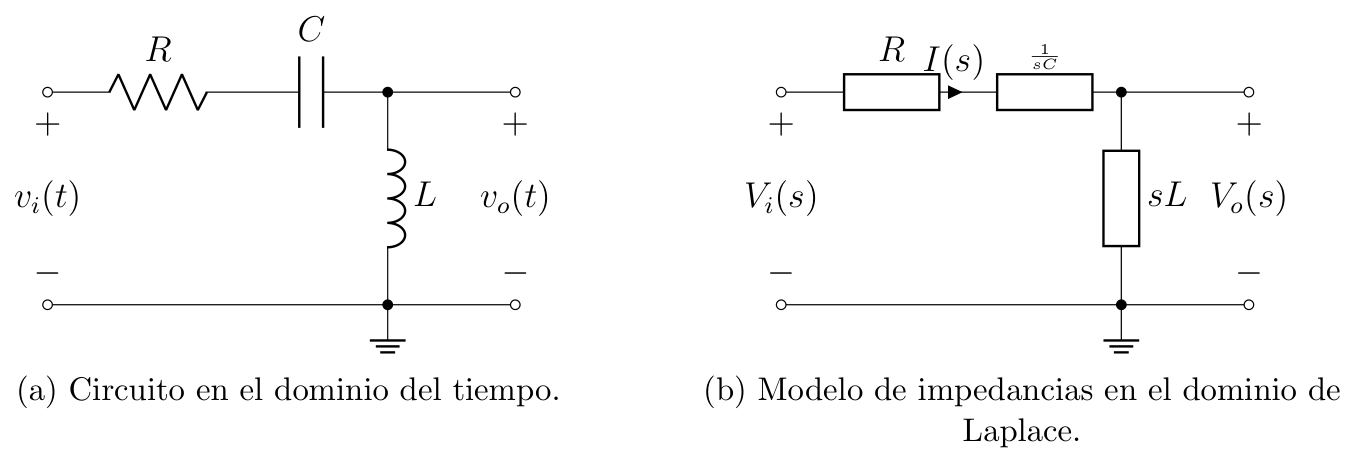
\includegraphics[width=\linewidth, height=3.6cm, keepaspectratio]{img/fig2_1_circuito_rlc.png}
      \vspace{4pt}
      \begin{tarjeta}[colframe=CardBorder, colback=CardBg, boxrule=0.5pt, top=3pt, bottom=3pt, left=5pt, right=5pt]
        {\fontsize{7.5pt}{9pt}\selectfont
        \textbf{\color{NavyDark} Parámetros del Circuito:} $R = \qty{100}{\ohm}$, $R_g = \qty{50}{\ohm}$, $R_t = \qty{150}{\ohm}$\\
        \textbf{\color{CyanDark} Salida:} $v_o(t)$ tomada directamente sobre el inductor $L$ a masa.
        }
      \end{tarjeta}
    \end{column}
  \end{columns}
\end{frame}

% SLIDE 6: DEDUCCIÓN DE TRANSFERENCIA
\subsection{Función de Transferencia}
\begin{frame}
  \frametitle{Deducción Matemática de $H(s)$ en Laplace}

  \begin{columns}[t, onlytextwidth]
    \begin{column}{0.48\textwidth}
      \begin{tarjeta}
        {\fontsize{9pt}{11pt}\selectfont \textbf{\color{NavyDark} Análisis de Malla en Laplace:}}\\[2pt]
        {\fontsize{8pt}{10pt}\selectfont
        Impedancia total de la malla serie:
        \[ Z_t(s) = R_t + sL + \frac{1}{sC} \]
        Corriente que circula por el circuito:
        \[ I(s) = \frac{V_i(s)}{Z_t(s)} = \frac{sC}{s^2 LC + sR_t C + 1} V_i(s) \]
        Tensión de salida tomada en el inductor $L$:
        \[ V_o(s) = sL \cdot I(s) \]
        }
      \end{tarjeta}
    \end{column}

    \begin{column}{0.48\textwidth}
      \begin{tarjeta}
        {\fontsize{9pt}{11pt}\selectfont \textbf{\color{NavyDark} Normalización de H(s):}}\\[2pt]
        {\fontsize{8pt}{10pt}\selectfont
        Dividiendo numerador y denominador por $LC$:
        \[ H(s) = \frac{V_o(s)}{V_i(s)} = \frac{s^2}{s^2 + s \frac{R_t}{L} + \frac{1}{LC}} \]
        \begin{itemize}\setlength{\itemsep}{2pt}
          \item \textbf{Numerador:} Cero doble en el origen ($s^2$).
          \item \textbf{Denominador:} Polinomio mónico de segundo orden que fija los polos del filtro.
        \end{itemize}
        }
      \end{tarjeta}
    \end{column}
  \end{columns}
\end{frame}

% SLIDE 7: FORMA CANÓNICA Y PROPIEDADES
\subsection{Forma Canónica y Propiedades}
\begin{frame}
  \frametitle{Forma Canónica de Segundo Orden y Parámetros}

  \begin{columns}[t, onlytextwidth]
    \begin{column}{0.48\textwidth}
      \begin{tarjeta}
        {\fontsize{9pt}{11pt}\selectfont \textbf{\color{NavyDark} Función Canónica Estándar:}}\\[2pt]
        {\fontsize{8pt}{10pt}\selectfont
        \[ H(s) = \frac{s^2}{s^2 + \frac{\omega_0}{Q} s + \omega_0^2} = \frac{s^2}{s^2 + 2\xi\omega_0 s + \omega_0^2} \]
        \begin{itemize}\setlength{\itemsep}{2pt}
          \item \textbf{Pulsación natural:} $\omega_0 = \frac{1}{\sqrt{LC}}$
          \item \textbf{Factor de calidad:} $Q = \frac{\omega_0 L}{R_t} = \frac{1}{R_t} \sqrt{\frac{L}{C}}$
          \item \textbf{Amortiguamiento:} $\xi = \frac{1}{2Q} = \frac{R_t}{2} \sqrt{\frac{C}{L}}$
        \end{itemize}
        }
      \end{tarjeta}
    \end{column}

    \begin{column}{0.48\textwidth}
      \begin{tarjeta}
        {\fontsize{9pt}{11pt}\selectfont \textbf{\color{NavyDark} Propiedades Frecuenciales:}}\\[2pt]
        {\fontsize{8pt}{10pt}\selectfont
        \begin{itemize}\setlength{\itemsep}{2.5pt}
          \item \textbf{Cero doble en el origen ($s=0$):}
          Genera una pendiente inicial de $+40\ \text{dB/década}$ ($+12\ \text{dB/octava}$) en banda atenuada.
          \item \textbf{Asíntota de alta frecuencia:}
          Para $\omega \gg \omega_0$, $H(j\omega) \to 1$ ($\qty{0}{\decibel}$, fase $\ang{0}$).
          \item \textbf{Fase en resonancia:}
          En $\omega = \omega_0$, la fase es exactamente $\ang{+90}$.
        \end{itemize}
        }
      \end{tarjeta}
    \end{column}
  \end{columns}
\end{frame}

% ==============================================================================
% BLOQUE 2: IGNACIO (NACHO) GIL (Slides 8 a 16 — 9 diapositivas)
% ==============================================================================

% SLIDE 8: EL DESAFÍO DE FRECUENCIA
\subsection{El Desafío de Frecuencia}
\begin{frame}
  \frametitle{Relación entre Pulsación Natural $\omega_0$ y Frecuencia de Corte $\omega_c$}

  \begin{columns}[t, onlytextwidth]
    \begin{column}{0.48\textwidth}
      \begin{tarjeta}
        {\fontsize{9pt}{11pt}\selectfont \textbf{\color{AlertAmber} Origen del Desvío en Frecuencia:}}\\[2pt]
        {\fontsize{8pt}{10pt}\selectfont
        \begin{itemize}\setlength{\itemsep}{2.5pt}
          \item $\omega_0 = \omega_c$ \textbf{únicamente} para Butterworth clásico ($Q = 1/\sqrt{2} \approx 0.707$).
          \item En la pulsación natural $\omega = \omega_0$:
          \[ |H(j\omega_0)| = Q \]
          \item Para $Q_1 = 0.25$: $|H(j\omega_0)| = 0.25 \implies \mathbf{-12.04\ \unit{\decibel}}$.
          Para alcanzar los $\qty{-3.01}{\decibel}$ de corte se debe subir en frecuencia ($\omega_c > \omega_0 \implies K < 1$).
          \item Para $Q_2 = 0.75$: $|H(j\omega_0)| = 0.75 \implies \mathbf{-2.50\ \unit{\decibel}}$.
          Supera los $\qty{-3.01}{\decibel}$, de modo que el corte ocurre antes ($\omega_c < \omega_0 \implies K > 1$).
        \end{itemize}
        }
      \end{tarjeta}
    \end{column}

    \begin{column}{0.48\textwidth}
      \begin{tarjeta}[colframe=BlueAccent]
        {\fontsize{9pt}{11pt}\selectfont \textbf{\color{BlueAccent} Introducción del Factor K:}}\\[2pt]
        {\fontsize{8pt}{10pt}\selectfont
        \begin{itemize}\setlength{\itemsep}{2.5pt}
          \item Se define la constante de corrección $K$:
          \[ \omega_0 = K \cdot \omega_c \]
          \item Permite fijar con exactitud analítica la frecuencia de corte a $\qty{-3.01}{\decibel}$ en $f_c = \qty{400}{\hertz}$.
          \item Relaciona la pulsación natural del filtro con la pulsación de corte especificada.
          \item Sin $K$, el filtro con $Q=0.25$ presentaría su corte en una frecuencia muy lejana a la solicitada.
        \end{itemize}
        }
      \end{tarjeta}
    \end{column}
  \end{columns}
\end{frame}

% SLIDE 9: DEDUCCIÓN DE K
\subsection{Deducción del Factor K}
\begin{frame}
  \frametitle{Deducción Analítica del Factor de Corrección $K$}

  \begin{columns}[t, onlytextwidth]
    \begin{column}{0.48\textwidth}
      \begin{tarjeta}
        {\fontsize{9pt}{11pt}\selectfont \textbf{\color{NavyDark} Condición a -3 dB: $|H|^2 = 1/2$}}\\[2pt]
        {\fontsize{8pt}{10pt}\selectfont
        Variable normalizada $x = \omega / \omega_0$:
        \[ |H(jx)|^2 = \frac{x^4}{(1 - x^2)^2 + \frac{x^2}{Q^2}} = \frac{1}{2} \]
        Llamando $a = 1 - \frac{1}{2Q^2}$ y como $K = 1/x_c$:
        \[ K = \sqrt{\left(1 - \frac{1}{2Q^2}\right) + \sqrt{\left(1 - \frac{1}{2Q^2}\right)^2 + 1}} \]
        (Expresión analítica exacta).
        }
      \end{tarjeta}
    \end{column}

    \begin{column}{0.48\textwidth}
      \begin{tarjeta}[colframe=NavyDark]
        {\fontsize{9pt}{11pt}\selectfont \textbf{\color{NavyDark} Valores Obtenidos ($f_c = \qty{400}{\hertz}$):}}\\[2pt]
        {\fontsize{8pt}{10pt}\selectfont
        \begin{itemize}\setlength{\itemsep}{3pt}
          \item \textbf{Caso 1 ($Q_1 = 0.25$):}
          $a = 1 - 8 = -7$\\
          $K_1 = \sqrt{-7 + \sqrt{50}} = \mathbf{0.2666}$\\
          $\omega_{0,1} = 2\pi \cdot 400 \cdot 0.2666 = \mathbf{\qty{670.0}{\radian\per\second}}$\\
          $f_{0,1} = \mathbf{\qty{106.6}{\hertz}}$
          \item \textbf{Caso 2 ($Q_2 = 0.75$):}
          $a = 1 - 0.8889 = 0.1111$\\
          $K_2 = \sqrt{0.1111 + \sqrt{1.0123}} = \mathbf{1.0570}$\\
          $\omega_{0,2} = 2\pi \cdot 400 \cdot 1.0570 = \mathbf{\qty{2656.5}{\radian\per\second}}$\\
          $f_{0,2} = \mathbf{\qty{422.8}{\hertz}}$
        \end{itemize}
        }
      \end{tarjeta}
    \end{column}
  \end{columns}
\end{frame}

% SLIDE 10: COMPONENTES
\subsection{Dimensionamiento}
\begin{frame}
  \frametitle{Dimensionamiento de Componentes ($R = \qty{100}{\ohm}$)}

  \begin{columns}[t, onlytextwidth]
    \begin{column}{0.48\textwidth}
      \begin{tarjeta}
        {\fontsize{9pt}{11pt}\selectfont \textbf{\color{NavyDark} Caso 1 ($Q_1 = 0.25$, $\omega_{0,1} = \qty{670.0}{\radian\per\second}$):}}\\[2pt]
        {\fontsize{8pt}{10pt}\selectfont
        \begin{itemize}\setlength{\itemsep}{2.5pt}
          \item Factor de corrección: $K_1 = \mathbf{0.2666}$.
          \item Frecuencia natural: $f_{0,1} = \mathbf{\qty{106.6}{\hertz}}$.
          \item Inductancia calculada ($R = \qty{100}{\ohm}$):\\
          $L_1 = \frac{R Q_1}{\omega_{0,1}} = \frac{100 \cdot 0.25}{670.0} = \mathbf{\qty{37.31}{\milli\henry}}$.
          \item Capacidad calculada:\\
          $C_1 = \frac{1}{\omega_{0,1} R Q_1} = \mathbf{\qty{59.70}{\micro\farad}}$.
          \item Factor de amortiguamiento:\\
          $\xi_1 = \frac{1}{2 Q_1} = \mathbf{2.000}$ (sobreamortiguado).
        \end{itemize}
        }
      \end{tarjeta}
    \end{column}

    \begin{column}{0.48\textwidth}
      \begin{tarjeta}[colframe=NavyDark]
        {\fontsize{9pt}{11pt}\selectfont \textbf{\color{NavyDark} Caso 2 ($Q_2 = 0.75$, $\omega_{0,2} = \qty{2656.5}{\radian\per\second}$):}}\\[2pt]
        {\fontsize{8pt}{10pt}\selectfont
        \begin{itemize}\setlength{\itemsep}{2.5pt}
          \item Factor de corrección: $K_2 = \mathbf{1.0570}$.
          \item Frecuencia natural: $f_{0,2} = \mathbf{\qty{422.8}{\hertz}}$.
          \item Inductancia calculada ($R = \qty{100}{\ohm}$):\\
          $L_2 = \frac{R Q_2}{\omega_{0,2}} = \frac{100 \cdot 0.75}{2656.5} = \mathbf{\qty{28.23}{\milli\henry}}$.
          \item Capacidad calculada:\\
          $C_2 = \frac{1}{\omega_{0,2} R Q_2} = \mathbf{\qty{5.02}{\micro\farad}}$.
          \item Factor de amortiguamiento:\\
          $\xi_2 = \frac{1}{2 Q_2} = \mathbf{0.667}$ (subamortiguado).
        \end{itemize}
        }
      \end{tarjeta}
    \end{column}
  \end{columns}
\end{frame}

% SLIDE 11: Q=0.25 POLOS
\subsection{Análisis Q = 0.25}
\begin{frame}
  \frametitle{Régimen Sobreamortiguado ($Q = 0.25$): Polos en Plano $s$}

  \begin{columns}[c, onlytextwidth]
    \begin{column}{0.44\textwidth}
      \begin{tarjeta}
        {\fontsize{9pt}{11pt}\selectfont \textbf{\color{NavyDark} Raíces Reales y Polo Dominante:}}\\[2pt]
        {\fontsize{7.5pt}{9.2pt}\selectfont
        \[ H_1(s) = \frac{s^2}{(s + 179.53)(s + 2500.72)} \]
        \begin{itemize}\setlength{\itemsep}{2pt}
          \item Con $\xi = 2.0 > 1$, discriminante positivo:
          $s_1 = \mathbf{-179.53\ \unit{\radian\per\second}}$ ($f_1 \approx \qty{28.6}{\hertz}$)\\
          $s_2 = \mathbf{-2500.72\ \unit{\radian\per\second}}$ ($f_2 \approx \qty{398.0}{\hertz}$)
          \item $s_1$ está $14$ veces más cerca del origen: actúa como el \textbf{polo dominante}.
          \item Constante de tiempo lenta: $\tau_1 = \frac{1}{|s_1|} = \mathbf{\qty{5.57}{\milli\second}}$.
        \end{itemize}
        }
      \end{tarjeta}
    \end{column}

    \begin{column}{0.54\textwidth}
      \centering
      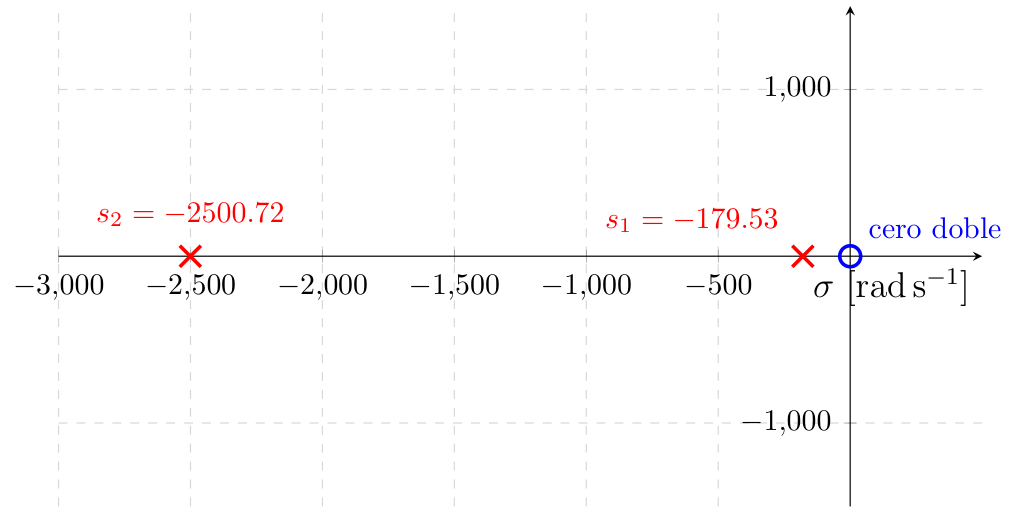
\includegraphics[width=\linewidth, height=3.6cm, keepaspectratio]{img/fig3_1_polos_q025.png}
      \vspace{3pt}
      \begin{tarjeta}[colframe=CardBorder, colback=CardBg, boxrule=0.5pt, top=3pt, bottom=3pt, left=5pt, right=5pt]
        {\fontsize{7.5pt}{9pt}\selectfont
        \textbf{\color{NavyDark} Dinámica Sobreamortiguada:} Dispersión de $14\times$ entre raíces ($s_1 = \mathbf{-179.5\ \text{rad/s}}$, $s_2 = -2500.7\ \text{rad/s}$). El polo lento $s_1$ gobierna el transitorio.
        }
      \end{tarjeta}
    \end{column}
  \end{columns}
\end{frame}

% SLIDE 12: Q=0.25 TEMPORAL
\begin{frame}
  \frametitle{Régimen Sobreamortiguado ($Q = 0.25$): Respuesta al Escalón}

  \begin{columns}[c, onlytextwidth]
    \begin{column}{0.44\textwidth}
      \begin{tarjeta}
        {\fontsize{9pt}{11pt}\selectfont \textbf{\color{NavyDark} Parámetros al Escalón Unitario:}}\\[2pt]
        {\fontsize{7.5pt}{9.2pt}\selectfont
        \[ v_o(t) = (1.0773 e^{-2500.7 t} - 0.0773 e^{-179.5 t}) u(t) \]
        \begin{itemize}\setlength{\itemsep}{2pt}
          \item \textbf{Valor inicial discontinuo:} $v_o(0^+) = \qty{1.0}{\volt}$.
          \item \textbf{Tiempo de caída ($\qty{90}{\percent}\to\qty{10}{\percent}$):} $\qty{0.70}{\milli\second}$.
          \item \textbf{Subpico máximo:} $\qty{-4.8}{\percent}$ (en $t = \qty{2.27}{\milli\second}$).
          \item \textbf{Tiempo de establecimiento ($\pm\qty{2}{\percent}$):}
          $t_s = \tau_1 \ln\left(\frac{0.0773}{0.02}\right) \approx \mathbf{\qty{7.53}{\milli\second}}$.
          \item Respuesta estrictamente aperiódica sin oscilación.
        \end{itemize}
        }
      \end{tarjeta}
    \end{column}

    \begin{column}{0.54\textwidth}
      \centering
      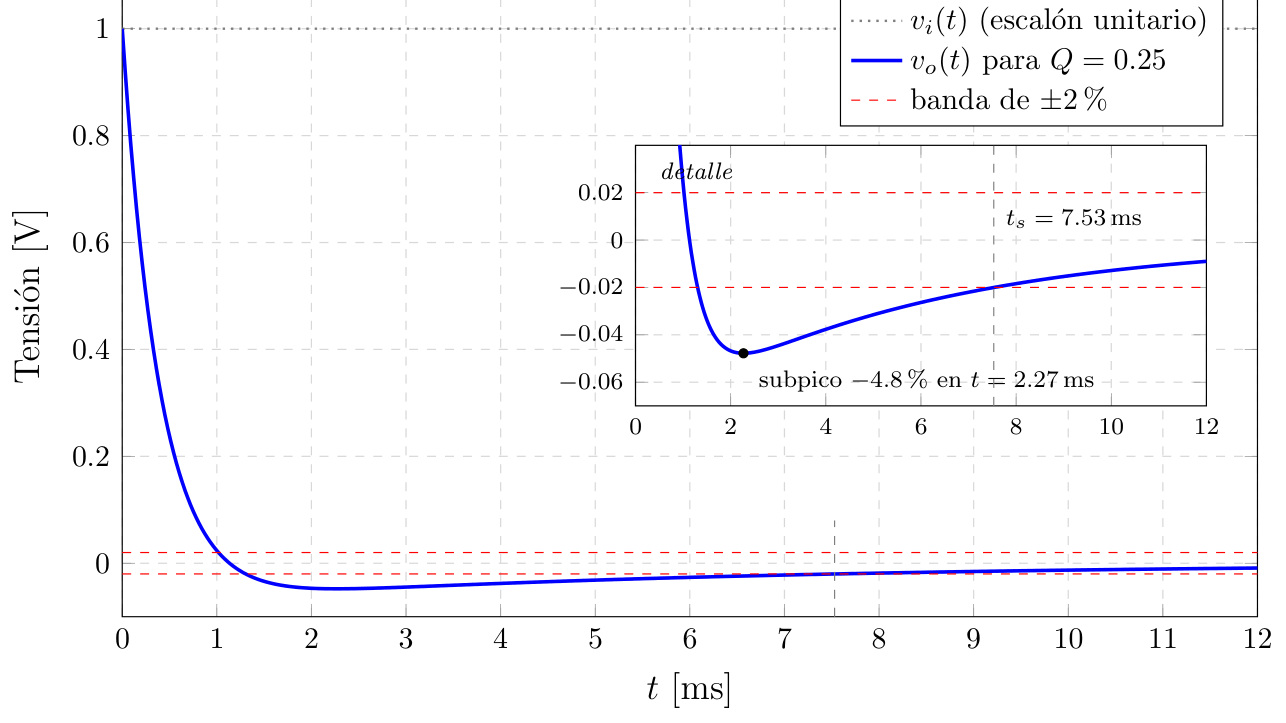
\includegraphics[width=\linewidth, height=3.6cm, keepaspectratio]{img/fig3_2_escalon_q025.png}
      \vspace{3pt}
      \begin{tarjeta}[colframe=CardBorder, colback=CardBg, boxrule=0.5pt, top=3pt, bottom=3pt, left=5pt, right=5pt]
        {\fontsize{7.5pt}{9pt}\selectfont
        \textbf{\color{NavyDark} Dinámica Aperiódica:} Respuesta estrictamente monótona sin oscilación. Subpico marginal de $\mathbf{-4.8\%}$ y establecimiento en $\mathbf{t_s = \qty{7.53}{\milli\second}}$.
        }
      \end{tarjeta}
    \end{column}
  \end{columns}
\end{frame}

% SLIDE 13: Q=0.75 POLOS
\subsection{Análisis Q = 0.75}
\begin{frame}
  \frametitle{Régimen Subamortiguado ($Q = 0.75$): Polos Complejos Conjugados}

  \begin{columns}[c, onlytextwidth]
    \begin{column}{0.46\textwidth}
      \begin{tarjeta}
        {\fontsize{9pt}{11pt}\selectfont \textbf{\color{NavyDark} Raíces Complejas en Plano s:}}\\[2pt]
        {\fontsize{7.5pt}{9.2pt}\selectfont
        \[ H_2(s) = \frac{s^2}{s^2 + 3542.33 s + 7056436} \]
        \begin{itemize}\setlength{\itemsep}{2pt}
          \item Con $\xi = 0.667 < 1$, discriminante negativo:
          $s_{1,2} = \mathbf{-1771.17 \pm j\, 1979.75\ \unit{\radian\per\second}}$.
          \item \textbf{Atenuación de envolvente:} $\sigma = \qty{1771.17}{\radian\per\second}$.
          \item \textbf{Pulsación amortiguada:}
          $\omega_d = \omega_0 \sqrt{1 - \xi^2} = \qty{1979.75}{\radian\per\second}$ ($f_d \approx \qty{315.1}{\hertz}$).
          \item Constante de envolvente: $\tau_2 = \mathbf{\qty{0.56}{\milli\second}}$ ($10\times$ más veloz).
        \end{itemize}
        }
      \end{tarjeta}
    \end{column}

    \begin{column}{0.52\textwidth}
      \centering
      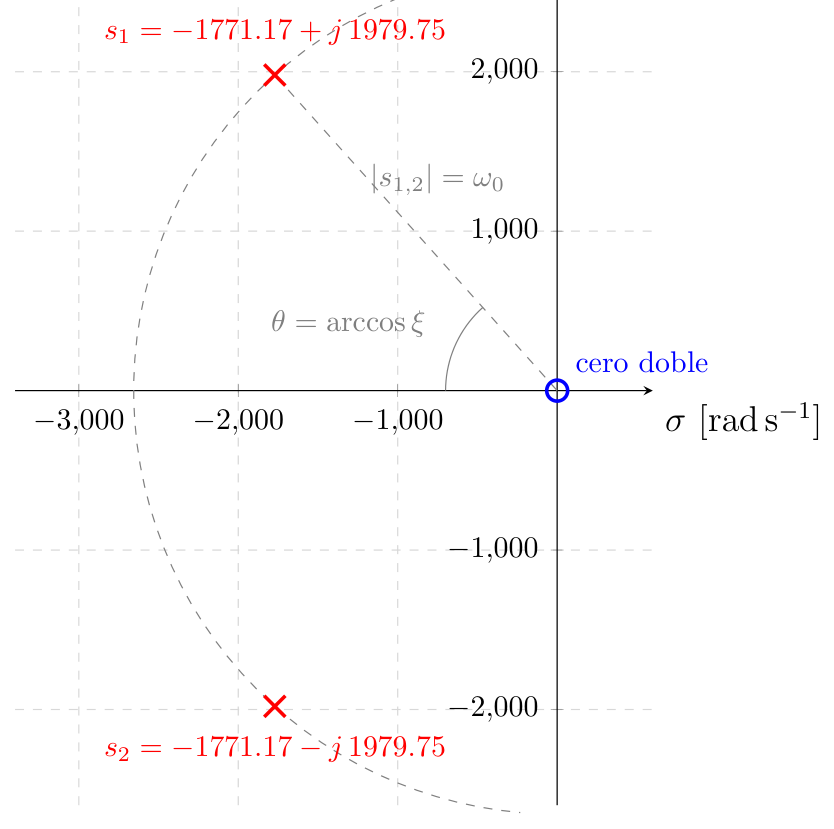
\includegraphics[width=\linewidth, height=5.2cm, keepaspectratio]{img/fig4_1_polos_q075.png}
    \end{column}
  \end{columns}
\end{frame}

% SLIDE 14: Q=0.75 TEMPORAL
\begin{frame}
  \frametitle{Régimen Subamortiguado ($Q = 0.75$): Respuesta Temporal y Subpico}

  \begin{columns}[c, onlytextwidth]
    \begin{column}{0.45\textwidth}
      \begin{tarjeta}
        {\fontsize{8.5pt}{10pt}\selectfont \textbf{\color{NavyDark} Parámetros al Escalón Unitario:}}\\[2pt]
        {\fontsize{7pt}{8.5pt}\selectfont
        \[ v_o(t) = e^{-\sigma t} [\cos(\omega_d t) - 0.8946 \sin(\omega_d t)] u(t) \]
        \begin{itemize}\setlength{\itemsep}{1.5pt}
          \item $\sigma = \qty{1771.17}{\radian\per\second}, \quad \omega_d = \qty{1979.75}{\radian\per\second}$.
          \item \textbf{Valor inicial discontinuo:} $v_o(0^+) = \qty{1.0}{\volt}$.
          \item \textbf{Tiempo de caída ($\qty{90}{\percent}\to\qty{10}{\percent}$):} $\qty{0.33}{\milli\second}$ ($2.1\times$ más rápido).
          \item \textbf{Primer cruce por cero:} $t_0 = \qty{0.425}{\milli\second}$.
          \item \textbf{Subpico máximo:} $\mathbf{\qty{-22.2}{\percent}}$ (en $t = \qty{0.85}{\milli\second}$).
          \item \textbf{Tiempo de establecimiento ($\pm\qty{2}{\percent}$):}
          $t_s = \mathbf{\qty{1.82}{\milli\second}}$ ($4.1\times$ más rápido).
          \item \textbf{Período de oscilación:} $T_d = \frac{2\pi}{\omega_d} = \qty{3.17}{\milli\second}$.
        \end{itemize}
        }
      \end{tarjeta}
    \end{column}

    \begin{column}{0.53\textwidth}
      \centering
      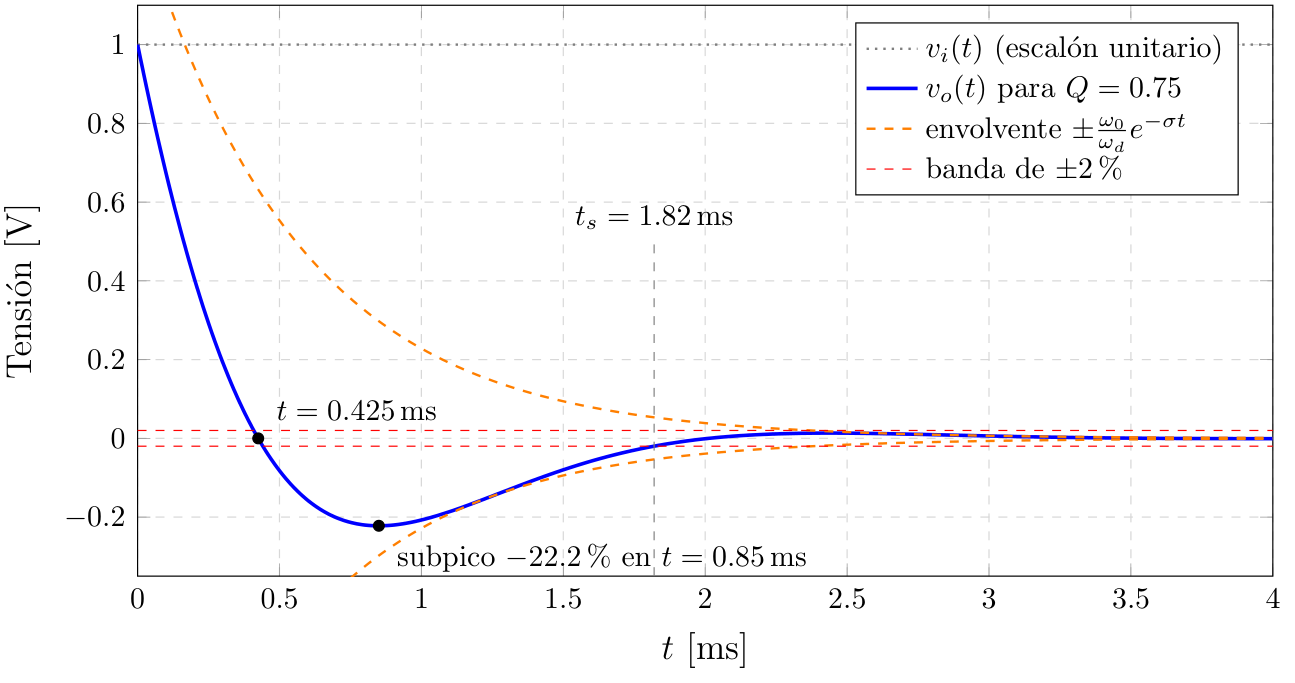
\includegraphics[width=\linewidth, height=3.6cm, keepaspectratio]{img/fig4_2_escalon_q075.png}
      \vspace{3pt}
      \begin{tarjeta}[colframe=CardBorder, colback=CardBg, boxrule=0.5pt, top=3pt, bottom=3pt, left=5pt, right=5pt]
        {\fontsize{7.5pt}{9pt}\selectfont
        \textbf{\color{AlertAmber} Dinámica Rápida Subamortiguada:} Recuperación en solo $\mathbf{t_s = \qty{1.82}{\milli\second}}$ ($4.1\times$ más veloz que $Q=0.25$) a costa de un subpico del $\mathbf{-22.2\%}$.
        }
      \end{tarjeta}
    \end{column}
  \end{columns}
\end{frame}

% SLIDE 15: COMPARATIVA TEMPORAL
\subsection{Comparativa Temporal}
\begin{frame}
  \frametitle{Comparativa Temporal Directa: $Q = 0.25$ vs $Q = 0.75$}

  \begin{columns}[c, onlytextwidth]
    \begin{column}{0.48\textwidth}
      \centering
      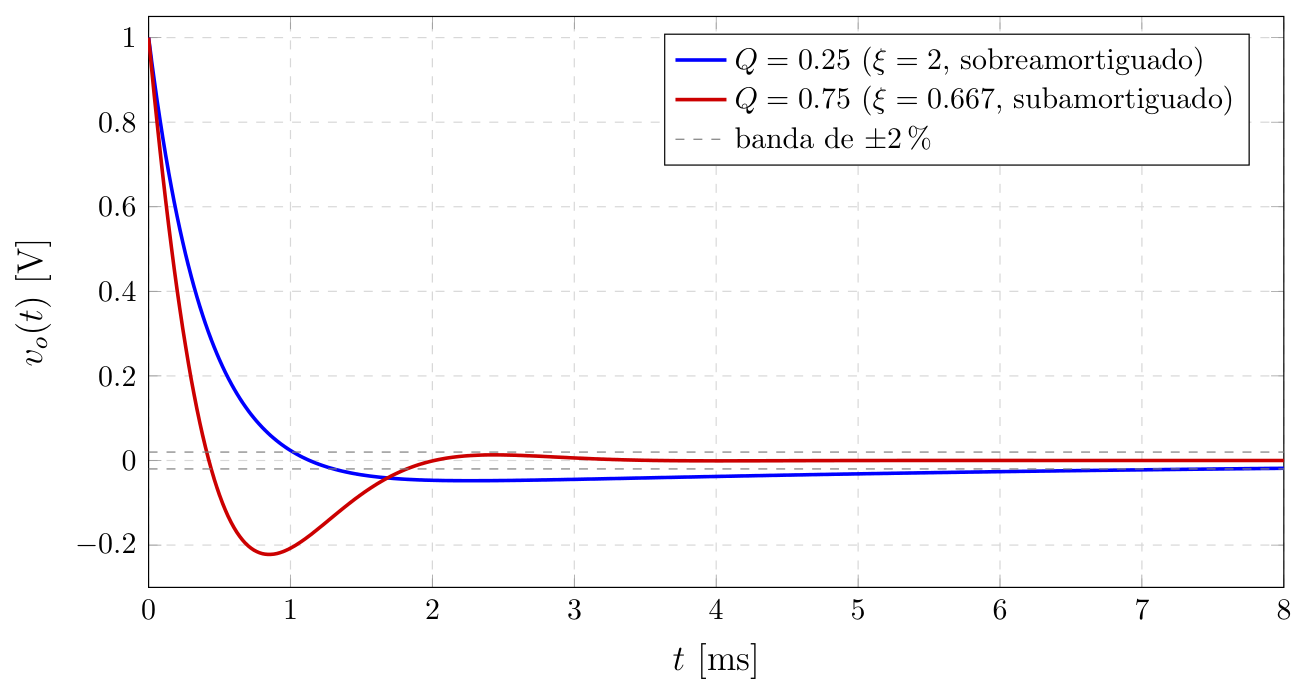
\includegraphics[width=\linewidth, height=3.5cm, keepaspectratio]{img/fig5_1_escalon_comparacion.png}
      \vspace{3pt}
      \begin{tarjeta}[colframe=CardBorder, colback=CardBg, boxrule=0.5pt, top=3pt, bottom=3pt, left=5pt, right=5pt]
        {\fontsize{7.5pt}{9pt}\selectfont
        \textbf{\color{NavyDark} Compromiso Fundamental:} $Q=0.75$ prioriza velocidad ($1.82\text{ ms}$) con oscilación; $Q=0.25$ asegura monotonía ($7.53\text{ ms}$) sin sobreimpulsos.
        }
      \end{tarjeta}
    \end{column}

    \begin{column}{0.50\textwidth}
      \begin{tarjeta}
        {\fontsize{8.5pt}{10pt}\selectfont \textbf{\color{NavyDark} Comparación de Parámetros Temporales:}}\\[2pt]
        \resizebox{\linewidth}{!}{%
        \setlength{\tabcolsep}{3pt}
        \renewcommand{\arraystretch}{1.05}
        {\fontsize{7pt}{8.5pt}\selectfont
        \begin{tabular}{lcc}
          \toprule
          \textbf{Parámetro} & \textbf{$Q = 0.25$} & \textbf{$Q = 0.75$} \\
          \midrule
          Factor amortiguamiento $\xi$ & $2.000$ & $0.667$ \\
          Tipo de amortiguamiento & Sobreamortiguado & Subamortiguado \\
          Raíces en plano $s$ & $-179.5\ ;\ -2500.7$ & $-1771.2 \pm j 1979.8$ \\
          Tiempo caída ($\qty{90}{\percent}\to\qty{10}{\percent}$) & $\qty{0.70}{\milli\second}$ & $\qty{0.33}{\milli\second}$ \\
          Subpico máximo & $\mathbf{-4.8\%}$ & $\mathbf{-22.2\%}$ \\
          Tiempo establecimiento ($2\%$) & $\qty{7.53}{\milli\second}$ & $\mathbf{\qty{1.82}{\milli\second}}$ \\
          Inductancia $L$ & $\qty{37.31}{\milli\henry}$ & $\qty{28.23}{\milli\henry}$ \\
          Capacidad $C$ & $\qty{59.70}{\micro\farad}$ & $\qty{5.02}{\micro\farad}$ \\
          \bottomrule
        \end{tabular}
        }%
        }
      \end{tarjeta}
    \end{column}
  \end{columns}
\end{frame}

% SLIDE 16: COMPARATIVA FRECUENCIAL
\subsection{Comparativa Frecuencial}
\begin{frame}
  \frametitle{Comparativa Frecuencial Directa: $Q = 0.25$ vs $Q = 0.75$}

  \begin{columns}[c, onlytextwidth]
    \begin{column}{0.56\textwidth}
      \centering
      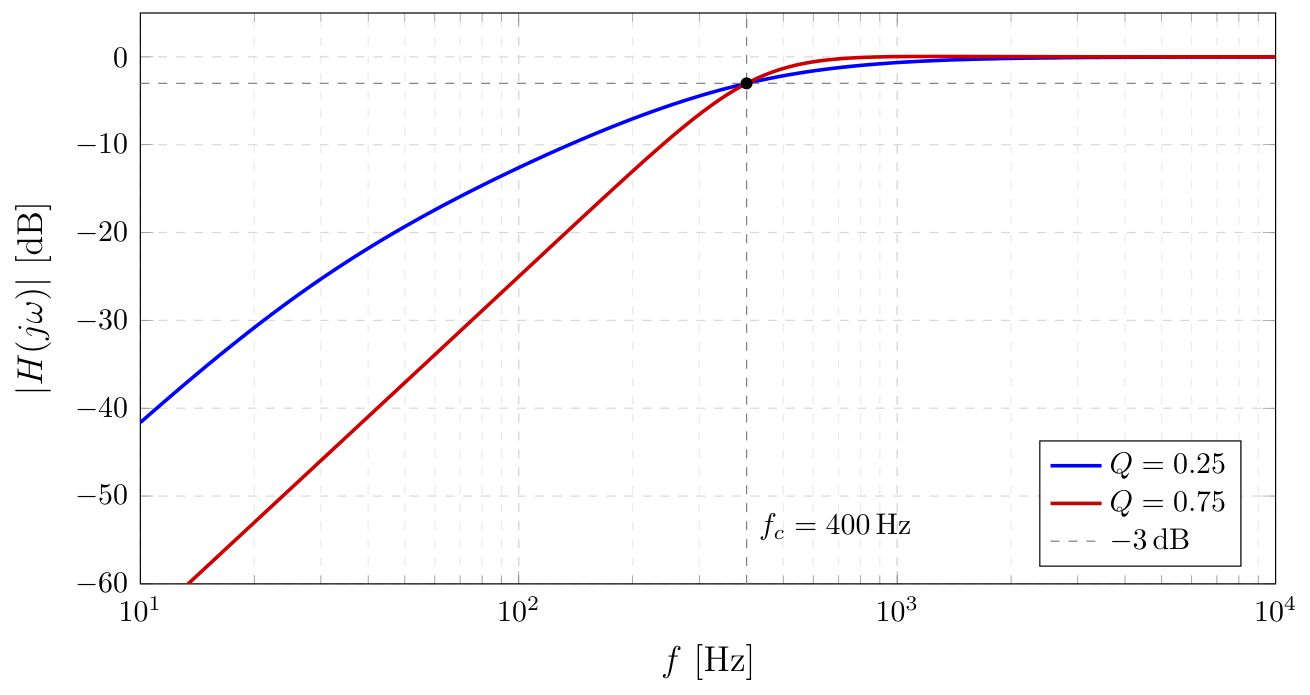
\includegraphics[width=\linewidth, height=4.8cm, keepaspectratio]{img/fig5_2_bode_comparacion.png}
    \end{column}

    \begin{column}{0.42\textwidth}
      \begin{tarjeta}
        {\fontsize{8.5pt}{10.5pt}\selectfont \textbf{\color{NavyDark} Contraste en Diagrama de Bode:}}\\[2pt]
        {\fontsize{7.5pt}{9.2pt}\selectfont
        \begin{itemize}\setlength{\itemsep}{2pt}
          \item \textbf{Pasa alto con $Q_1 = 0.25$:}
          Rodilla de transición muy suave y redondeada. Atenuación prematura en la cercanía de la banda de paso.
          \item \textbf{Pasa alto con $Q_2 = 0.75$:}
          Transición abrupta y selectiva en torno a $f_c = \qty{400}{\hertz}$. Mantiene mayor ganancia en banda útil.
          \item \textbf{Conclusión de diseño:}
          $Q=0.25$ es mandatorio ante tolerancia nula a oscilaciones; $Q=0.75$ es superior para filtrado rápido y selectivo.
        \end{itemize}
        }
      \end{tarjeta}
    \end{column}
  \end{columns}
\end{frame}

% ==============================================================================
% BLOQUE 3: ANGELO PRIETO (Slides 17 a 24 — 8 diapositivas)
% ==============================================================================

% SLIDE 17: PLANTA DE 3ER ORDEN
\section{Compensación de Sistemas}
\subsection{Planta de 3er Orden}
\begin{frame}
  \frametitle{Planta de Tercer Orden y Parámetros}

  \begin{columns}[t, onlytextwidth]
    \begin{column}{0.48\textwidth}
      \begin{tarjeta}
        {\fontsize{9pt}{11pt}\selectfont \textbf{\color{NavyDark} Función de Transferencia:}}\\[2pt]
        {\fontsize{8pt}{10pt}\selectfont
        \[ G(s) = \frac{K}{\left(1 + \frac{s}{p_1}\right)\left(1 + \frac{s}{p_2}\right)\left(1 + \frac{s}{p_3}\right)} \]
        \begin{itemize}\setlength{\itemsep}{2.5pt}
          \item \textbf{Ganancia estática en continua:}
          $K = 900 \implies |G(0)| = \mathbf{\qty{59.08}{\decibel}}$.
          \item \textbf{Ancho de banda base ($BW_{\text{LA}}$):}
          $BW = f_{-3\text{dB}} \approx \mathbf{\qty{11.59}{\kilo\hertz}}$.
          \item Dominado por el primer polo de $12\text{ kHz}$.
        \end{itemize}
        }
      \end{tarjeta}
    \end{column}

    \begin{column}{0.48\textwidth}
      \begin{tarjeta}
        {\fontsize{9pt}{11pt}\selectfont \textbf{\color{NavyDark} Polos Asignados (Grupo 5):}}\\[2pt]
        {\fontsize{8pt}{10pt}\selectfont
        \begin{itemize}\setlength{\itemsep}{3pt}
          \item \textbf{Primer polo ($f_{p1}$):}
          $f_{p1} = \qty{12}{\kilo\hertz} \implies p_1 \approx \qty{75398}{\radian\per\second}$
          \item \textbf{Segundo polo ($f_{p2}$):}
          $f_{p2} = \qty{70}{\kilo\hertz} \implies p_2 \approx \qty{439823}{\radian\per\second}$
          \item \textbf{Tercer polo ($f_{p3}$):}
          $f_{p3} = \qty{140}{\kilo\hertz} \implies p_3 \approx \qty{879646}{\radian\per\second}$
          \item Planta de orden 3 con alta ganancia y polos en alta frecuencia.
        \end{itemize}
        }
      \end{tarjeta}
    \end{column}
  \end{columns}
\end{frame}

% SLIDE 18: ANÁLISIS DE BODE
\subsection{Respuesta en Frecuencia}
\begin{frame}
  \frametitle{Respuesta en Frecuencia a Lazo Abierto (Bode)}

  \begin{columns}[c, onlytextwidth]
    \begin{column}{0.58\textwidth}
      \centering
      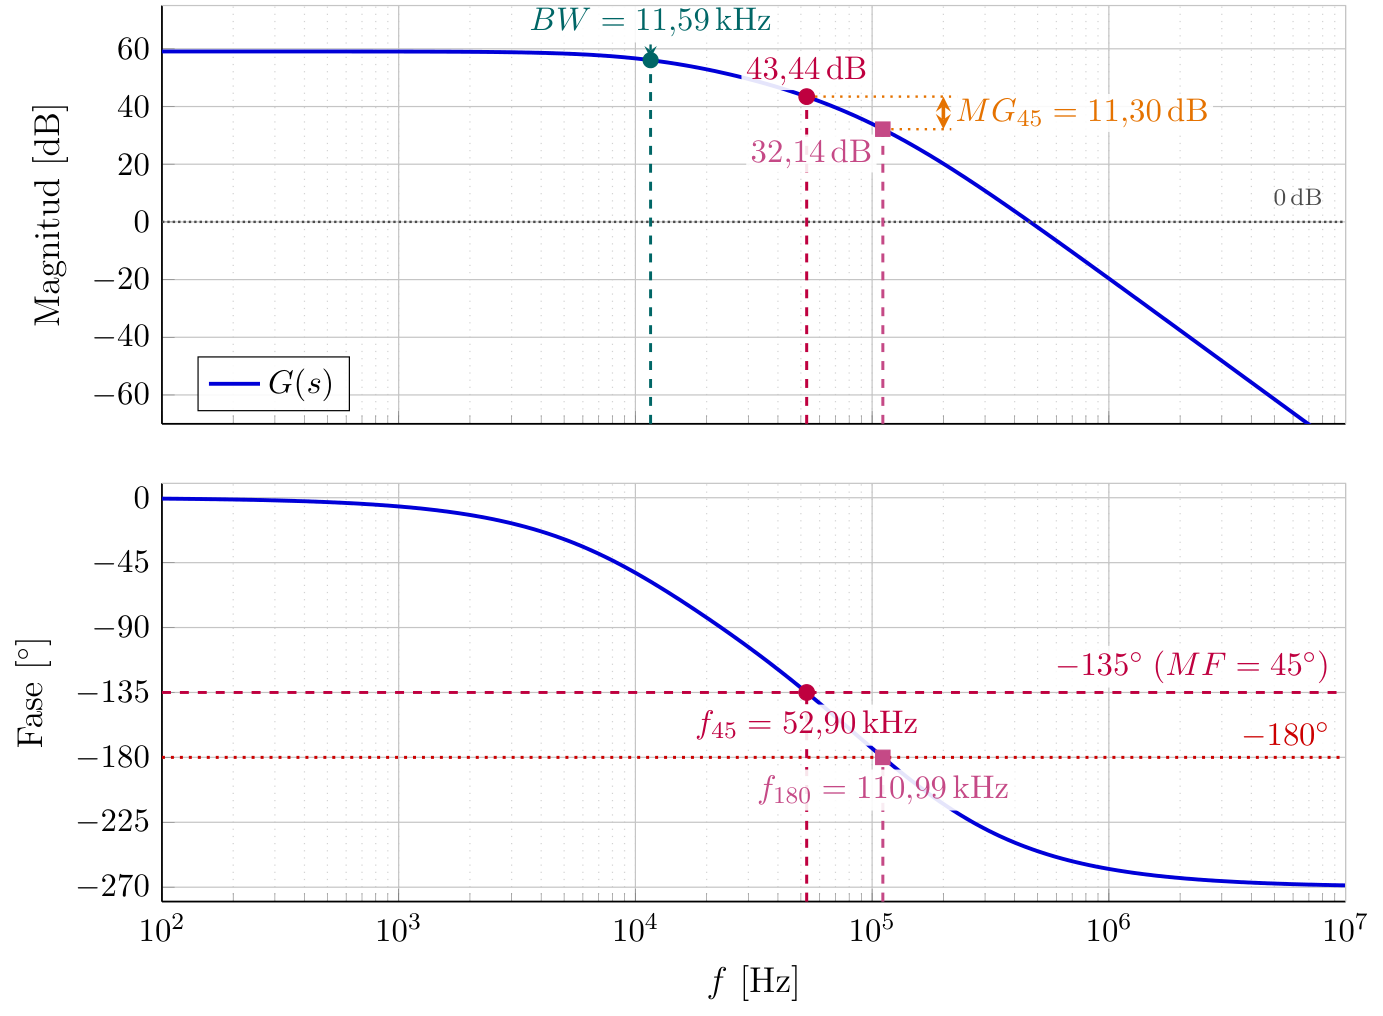
\includegraphics[width=\linewidth, height=5.5cm, keepaspectratio]{img/fig6_1_bode_planta.png}
    \end{column}

    \begin{column}{0.40\textwidth}
      \begin{tarjeta}
        {\fontsize{8.5pt}{10pt}\selectfont \textbf{\color{NavyDark} Comportamiento Asintótico:}}\\[2pt]
        {\fontsize{7pt}{8.5pt}\selectfont
        \begin{itemize}\setlength{\itemsep}{2pt}
          \item \textbf{$f < 12\text{ kHz}$:} Ganancia $+59.08\text{ dB}$, fase $\ang{0}$.
          \item \textbf{$12\text{k} < f < 70\text{ kHz}$:} Actúa $p_1$; pendiente $-20\ \text{dB/década}$, fase hacia $\ang{-90}$.
          \item \textbf{$70\text{k} < f < 140\text{ kHz}$:} Actúan $p_1, p_2$; pendiente $-40\ \text{dB/década}$, cruce por $\ang{-180}$.
          \item \textbf{$f > 140\text{ kHz}$:} Actúan 3 polos; pendiente $-60\ \text{dB/década}$, fase hacia $\ang{-270}$.
        \end{itemize}
        }
      \end{tarjeta}
    \end{column}
  \end{columns}
\end{frame}

% SLIDE 19: DIAGNÓSTICO DE INESTABILIDAD
\subsection{Diagnóstico de Inestabilidad}
\begin{frame}
  \frametitle{Diagnóstico de Inestabilidad a Lazo Cerrado}

  \begin{columns}[t, onlytextwidth]
    \begin{column}{0.48\textwidth}
      \begin{tarjeta}[colframe=AlertRed]
        {\fontsize{9pt}{11pt}\selectfont \textbf{\color{AlertRed} Diagnóstico Numérico Directo:}}\\[2pt]
        {\fontsize{8pt}{10pt}\selectfont
        \begin{itemize}\setlength{\itemsep}{2.5pt}
          \item \textbf{Cruce de fase por $\ang{-180}$:}
          $f_{180} \approx \mathbf{\qty{110.99}{\kilo\hertz}}$
          \item \textbf{Ganancia en el cruce de fase:}
          $|G(f_{180})| \approx \mathbf{\qty{32.14}{\decibel}}$ ($40.5$ veces)
          \item \textbf{Margen de Ganancia directo:}
          $MG = 0 - 32.14 = \mathbf{-32.14\ \unit{\decibel}}$
          \item \textbf{Cruce de ganancia por $\qty{0}{\decibel}$:}
          $f_{0\si{\decibel}} \approx \qty{464.42}{\kilo\hertz}$ con fase $\ang{-243.17}$ ($MF = \ang{-63.17}$).
        \end{itemize}
        }
      \end{tarjeta}
    \end{column}

    \begin{column}{0.48\textwidth}
      \begin{tarjeta}
        {\fontsize{9pt}{11pt}\selectfont \textbf{\color{NavyDark} Consecuencia Física:}}\\[2pt]
        {\fontsize{8pt}{10pt}\selectfont
        \begin{itemize}\setlength{\itemsep}{2.5pt}
          \item Con realimentación unitaria directa, la planta es \textbf{incondicionalmente inestable}.
          \item En $110.99\text{ kHz}$ el desfasaje de $\ang{-180}$ transforma la realimentación negativa en positiva con amplificación de $40.5$ veces.
          \item Los polos de lazo cerrado migran al semiplano derecho $\to$ auto-oscilación violenta.
          \item \textbf{Solución:} Es mandatorio diseñar redes de compensación en frecuencia.
        \end{itemize}
        }
      \end{tarjeta}
    \end{column}
  \end{columns}
\end{frame}

% SLIDE 20: CALIBRACIÓN MF = 45°
\subsection{Calibración para MF = 45°}
\begin{frame}
  \frametitle{Criterio de Calibración para Margen de Fase $MF = \ang{45}$}

  \begin{columns}[c, onlytextwidth]
    \begin{column}{0.48\textwidth}
      \begin{tarjeta}[colframe=AlertGreen]
        {\fontsize{9pt}{11pt}\selectfont \textbf{\color{AlertGreen} Determinación Gráfica en Bode:}}\\[2pt]
        {\fontsize{8pt}{10pt}\selectfont
        \begin{itemize}\setlength{\itemsep}{2.5pt}
          \item \textbf{Fase requerida para $MF = \ang{45}$:}
          $\phi = \ang{-180} + \ang{45} = \mathbf{\ang{-135}}$
          \item \textbf{Frecuencia para $\phi = \ang{-135}$ ($f_{45}$):}
          $f_{45} \approx \mathbf{\qty{52.90}{\kilo\hertz}}$
          \item \textbf{Ganancia disponible en $f_{45}$:}
          $|G(f_{45})| \approx \mathbf{\qty{43.44}{\decibel}}$ ($148.6$ veces)
          \item \textbf{Margen de Ganancia disponible ($MG_{45}$):}
          $MG_{45} = 43.44 - 32.14 = \mathbf{11.30\ \unit{\decibel}} > \qty{6}{\decibel}$
        \end{itemize}
        }
      \end{tarjeta}
    \end{column}

    \begin{column}{0.48\textwidth}
      \begin{tarjeta}
        {\fontsize{9pt}{11pt}\selectfont \textbf{\color{NavyDark} Significado en Diseño:}}\\[2pt]
        {\fontsize{8pt}{10pt}\selectfont
        \begin{itemize}\setlength{\itemsep}{2.5pt}
          \item Atenuar puramente con un divisor resistivo exigiría $\beta = 1/148.6 = \qty{-43.44}{\decibel}$.
          \item $MG_{45} = \qty{11.30}{\decibel} > \qty{6}{\decibel}$ garantiza que la planta admite operar con $MF = \ang{45}$ manteniendo margen seguro.
          \item Se abordarán dos estrategias pasivas:
          \begin{itemize}\setlength{\itemsep}{1.5pt}
            \item Compensador de Retardo (Lag).
            \item Red de Atraso-Adelanto (Lead-Lag).
          \end{itemize}
        \end{itemize}
        }
      \end{tarjeta}
    \end{column}
  \end{columns}
\end{frame}

% SLIDE 21: RETARDO SÍNTESIS
\subsection{Compensador de Retardo}
\begin{frame}
  \frametitle{Síntesis del Compensador de Retardo (Lag)}

  \begin{columns}[c, onlytextwidth]
    \begin{column}{0.48\textwidth}
      \begin{tarjeta}
        {\fontsize{8.5pt}{10.5pt}\selectfont \textbf{\color{NavyDark} Topología y Dimensionamiento:}}\\[2pt]
        {\fontsize{7.5pt}{9.2pt}\selectfont
        \[ G_c(s) = \frac{1}{1 + sRC} = \frac{1}{1 + \frac{s}{2\pi f_d}}, \quad f_d = \qty{1.2}{\kilo\hertz} \]
        \begin{itemize}\setlength{\itemsep}{2pt}
          \item Capacitor comercial adoptado: $C = \mathbf{\qty{100}{\nano\farad}}$ (film).
          \item Resistencia calculada:
          $R = \frac{1}{2\pi f_d C} \approx \qty{1326.29}{\ohm}$.
          \item \textbf{Normalización comercial ($\qty{1}{\percent}$):}
          $R = \mathbf{\qty{1.33}{\kilo\ohm}}$ (Serie E96).
          \item \textbf{Principio del Polo Dominante:}
          El polo en $1.2\text{ kHz}$ derriba la ganancia antes de que los polos en $70\text{k}$ y $140\text{ kHz}$ aporten desfasaje.
        \end{itemize}
        }
      \end{tarjeta}
    \end{column}

    \begin{column}{0.50\textwidth}
      \centering
      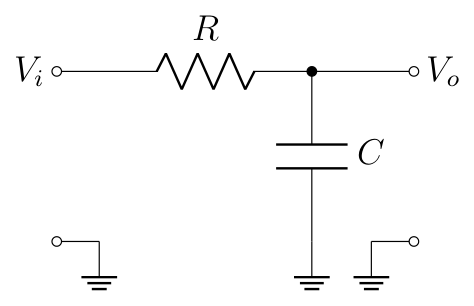
\includegraphics[width=\linewidth, height=4.6cm, keepaspectratio]{img/fig6_2_circuito_retardo.png}
    \end{column}
  \end{columns}
\end{frame}

% SLIDE 22: RETARDO BODE
\begin{frame}
  \frametitle{Compensador de Retardo: Respuesta y Pérdida de Ancho de Banda}

  \begin{columns}[c, onlytextwidth]
    \begin{column}{0.58\textwidth}
      \centering
      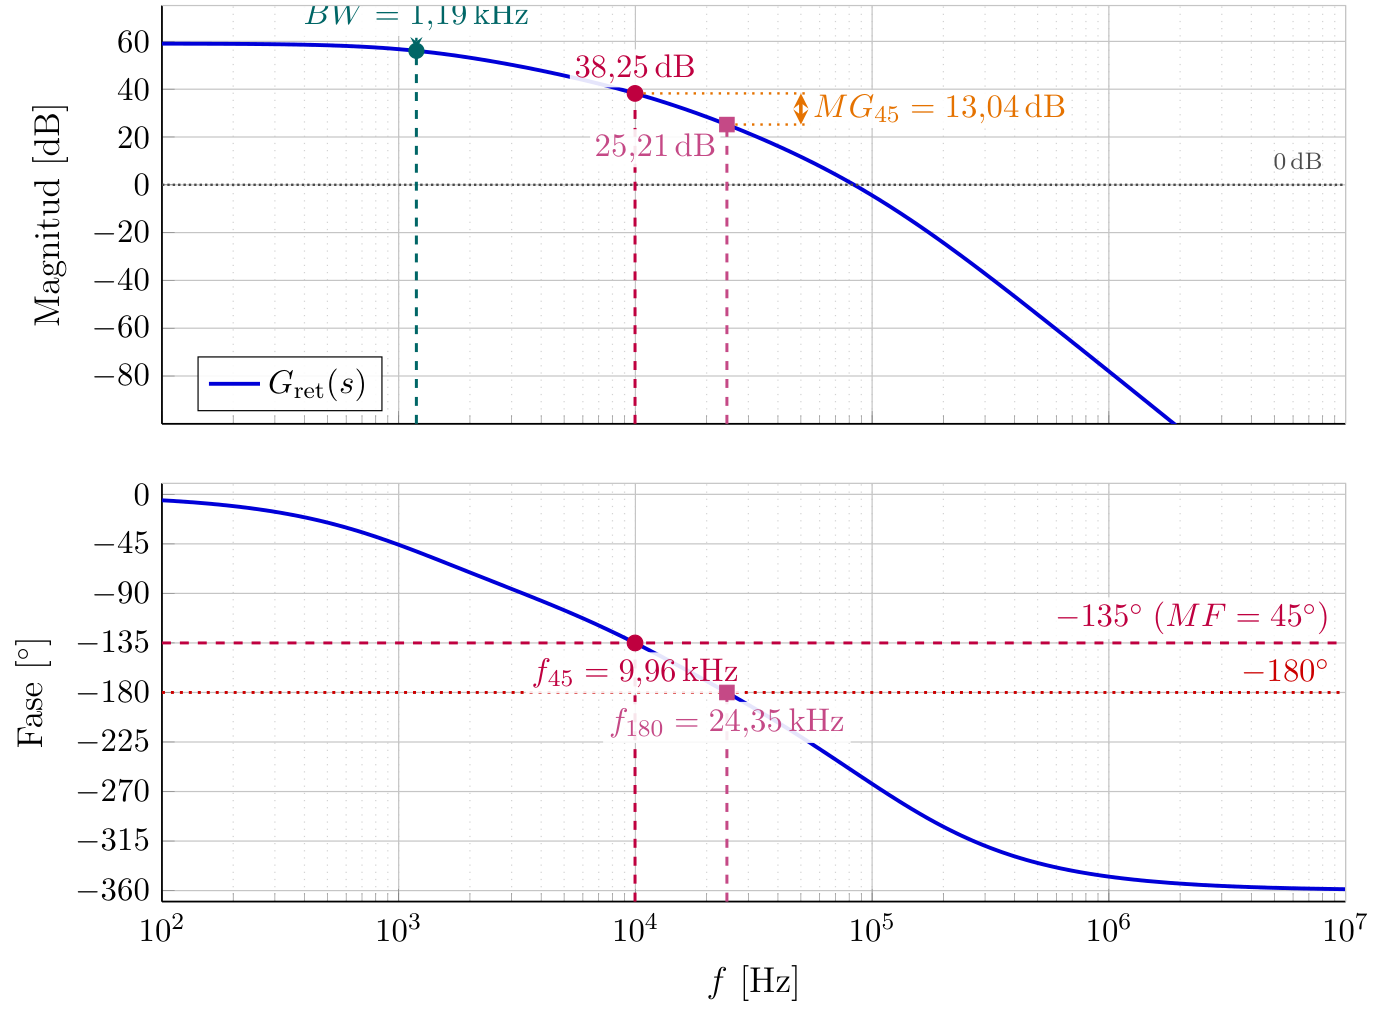
\includegraphics[width=\linewidth, height=5.5cm, keepaspectratio]{img/fig6_3_bode_retardo.png}
    \end{column}

    \begin{column}{0.40\textwidth}
      \begin{tarjeta}
        {\fontsize{8.5pt}{10pt}\selectfont \textbf{\color{NavyDark} Parámetros (MF = 45°):}}\\[2pt]
        {\fontsize{7pt}{8.5pt}\selectfont
        \begin{itemize}\setlength{\itemsep}{2pt}
          \item \textbf{Colapso de ancho de banda:}\\
          $BW = f_{-3\text{dB}} \approx \mathbf{\qty{1.19}{\kilo\hertz}}$\\
          (pérdida del $\mathbf{89.7\%}$ de banda útil).
          \item \textbf{Frecuencia para $MF = \ang{45}$:}\\
          $f_{45} \approx \qty{9.96}{\kilo\hertz}$ ($|G| \approx \qty{38.25}{\decibel}$).
          \item \textbf{Cruce por $\ang{-180}$:}\\
          $f_{180} \approx \qty{24.35}{\kilo\hertz}$ ($|G| \approx \qty{25.21}{\decibel}$).
          \item \textbf{Margen de Ganancia disponible:}\\
          $MG_{45} = \mathbf{13.04\ \unit{\decibel}} > \qty{6}{\decibel}$.
        \end{itemize}
        }
      \end{tarjeta}
    \end{column}
  \end{columns}
\end{frame}

% SLIDE 23: ATRASO-ADELANTO ESTRUCTURA
\subsection{Compensador de Atraso-Adelanto}
\begin{frame}
  \frametitle{Red de Atraso-Adelanto: Estructura Topológica}

  \begin{columns}[c, onlytextwidth]
    \begin{column}{0.48\textwidth}
      \begin{tarjeta}
        {\fontsize{8.5pt}{10.5pt}\selectfont \textbf{\color{NavyDark} Topología Circuital y Objetivos:}}\\[2pt]
        {\fontsize{7.5pt}{9.2pt}\selectfont
        \begin{itemize}\setlength{\itemsep}{2pt}
          \item \textbf{Estructura:} Rama serie con $R_1$, y rama derivación con $R_2$ en serie con $C$.
          \item \textbf{Función de transferencia de la red:}
          \[ G_{c2}(s) = \frac{1 + s R_2 C}{1 + s (R_1 + R_2) C} = \frac{1 + \frac{s}{2\pi f_z}}{1 + \frac{s}{2\pi f_p}} \]
          \item \textbf{Frecuencias asignadas:}
          Polo $f_p = \qty{220}{\kilo\hertz}$, Cero $f_z = \qty{1.1}{\mega\hertz}$.
          \item \textbf{Preservación de Banda Base:}
          Como $f_p, f_z \gg 12\text{ kHz}$, la banda base útil permanece inalterada.
        \end{itemize}
        }
      \end{tarjeta}
    \end{column}

    \begin{column}{0.50\textwidth}
      \centering
      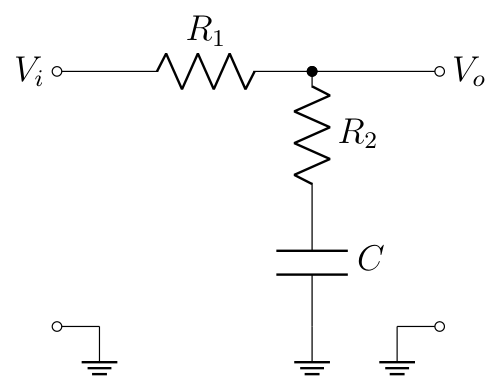
\includegraphics[width=\linewidth, height=4.8cm, keepaspectratio]{img/fig6_4_circuito_aa.png}
    \end{column}
  \end{columns}
\end{frame}

% SLIDE 24: ATRASO-ADELANTO BODE Y RESULTADOS
\begin{frame}
  \frametitle{Red de Atraso-Adelanto: Respuesta y Preservación de Ancho de Banda}

  \begin{columns}[c, onlytextwidth]
    \begin{column}{0.58\textwidth}
      \centering
      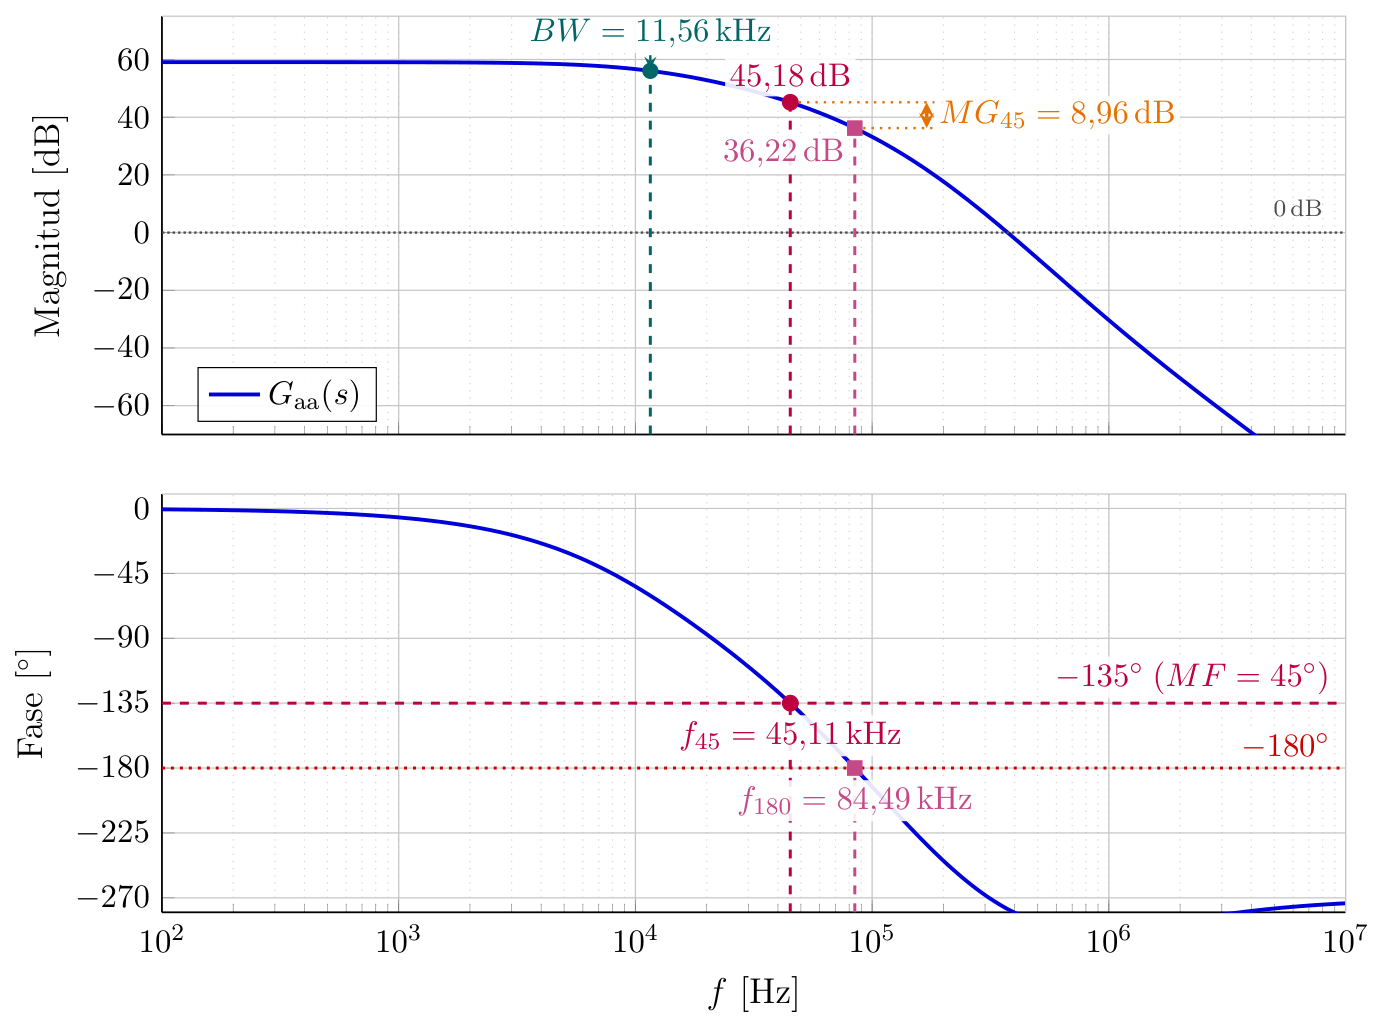
\includegraphics[width=\linewidth, height=5.5cm, keepaspectratio]{img/fig6_5_bode_aa.png}
    \end{column}

    \begin{column}{0.40\textwidth}
      \begin{tarjeta}
        {\fontsize{8.5pt}{10pt}\selectfont \textbf{\color{NavyDark} Componentes y Desempeño:}}\\[2pt]
        {\fontsize{7pt}{8.5pt}\selectfont
        \begin{itemize}\setlength{\itemsep}{2pt}
          \item \textbf{Componentes ($C = \qty{100}{\pico\farad}$ C0G):}\\
          $R_2 = \mathbf{\qty{1.45}{\kilo\ohm}}$, $R_1 = \mathbf{\qty{5.76}{\kilo\ohm}}$ ($\qty{1}{\percent}$).
          \item \textbf{Ancho de banda preservado:}\\
          $BW \approx \mathbf{\qty{11.56}{\kilo\hertz}}$ ($\mathbf{99.7\%}$).
          \item \textbf{Frecuencia para $MF = \ang{45}$:}\\
          $f_{45} \approx \mathbf{\qty{45.11}{\kilo\hertz}}$ ($4.5\times$ más veloz).
          \item \textbf{Margen de Ganancia disponible:}\\
          $MG_{45} = \mathbf{8.96\ \unit{\decibel}} > \qty{6}{\decibel}$.
        \end{itemize}
        }
      \end{tarjeta}
    \end{column}
  \end{columns}
\end{frame}

% ==============================================================================
% BLOQUE 4: GASTÓN GRASSO (Slides 25 a 32 — 8 diapositivas)
% ==============================================================================

% SLIDE 25: SUPERPOSICIÓN DE BODES
\section{Comparativa y Cierre}
\subsection{Superposición de Bodes}
\begin{frame}
  \frametitle{Comparativa de Bodes: Planta Original vs Compensadores}

  \begin{columns}[c, onlytextwidth]
    \begin{column}{0.58\textwidth}
      \centering
      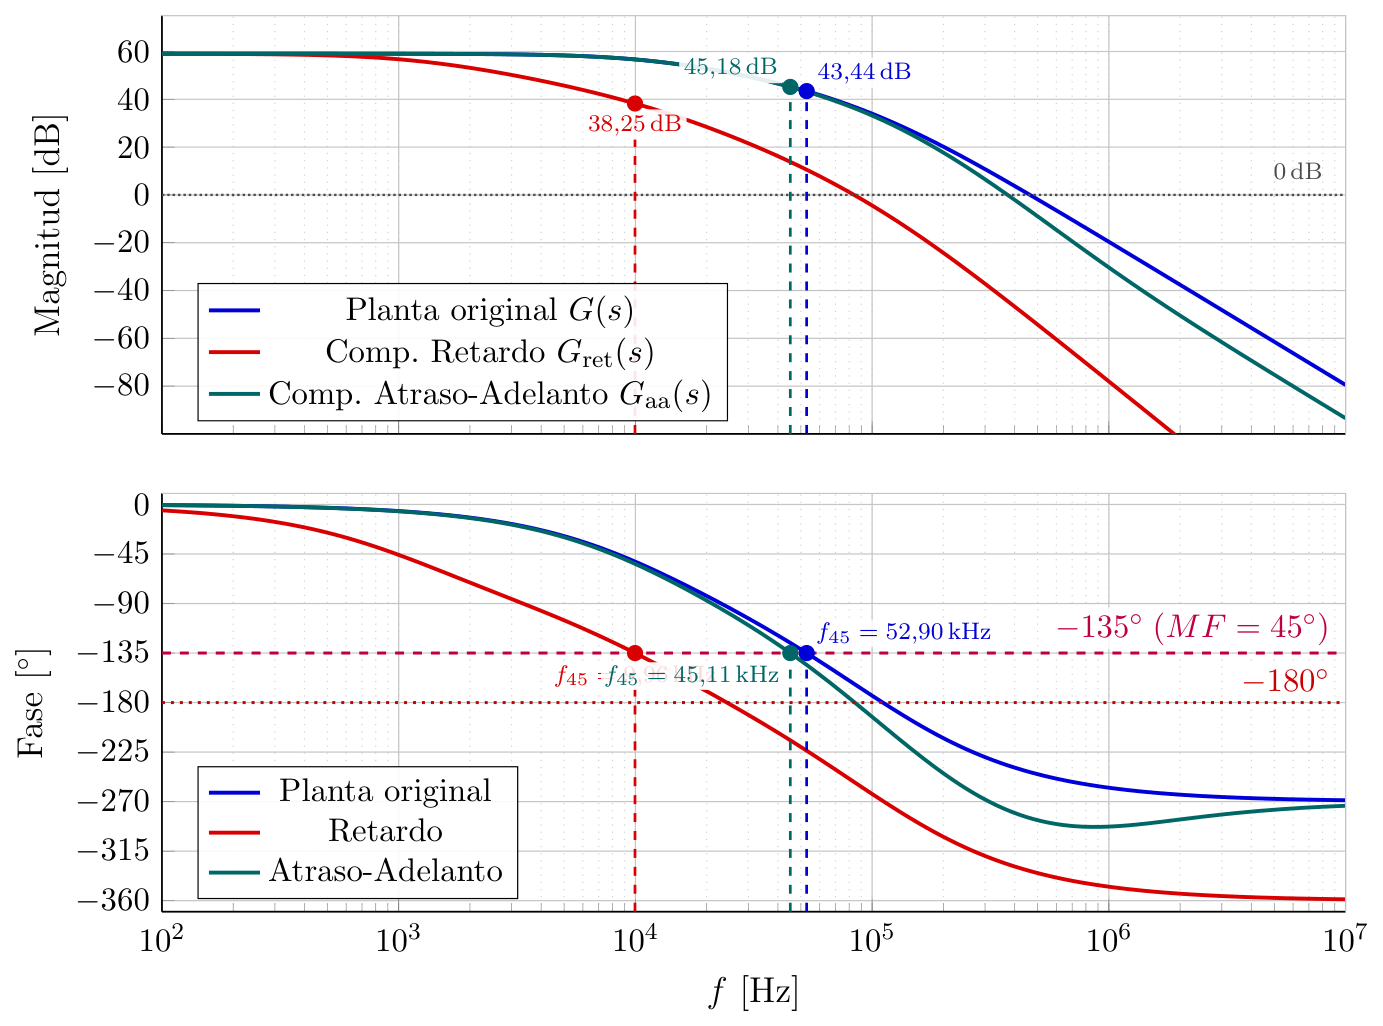
\includegraphics[width=\linewidth, height=5.5cm, keepaspectratio]{img/fig6_6_bode_comparativa.png}
    \end{column}

    \begin{column}{0.40\textwidth}
      \begin{tarjeta}
        {\fontsize{8.5pt}{10pt}\selectfont \textbf{\color{NavyDark} Análisis Visual Comparativo:}}\\[2pt]
        {\fontsize{7pt}{8.5pt}\selectfont
        \begin{itemize}\setlength{\itemsep}{2pt}
          \item \textbf{Curva Azul:} Planta original ($BW = \qty{11.59}{\kilo\hertz}$).
          \item \textbf{Curva Roja:} Retardo. Caída prematura desde $1.2\text{ kHz}$; contrae el ancho de banda a $\qty{1.19}{\kilo\hertz}$ (pérdida del $\qty{89.7}{\percent}$).
          \item \textbf{Curva Verde:} Atraso-Adelanto. Preserva la respuesta útil ($BW = \qty{11.56}{\kilo\hertz}$) y atenúa únicamente en alta frecuencia.
        \end{itemize}
        }
      \end{tarjeta}
    \end{column}
  \end{columns}
\end{frame}

% SLIDE 26: CUADRO COMPARATIVO CUANTITATIVO
\subsection{Cuadro Comparativo}
\begin{frame}
  \frametitle{Cuadro Comparativo Cuantitativo Integral (MF = 45°)}

  \begin{tarjeta}
    \centering
    \setlength{\tabcolsep}{3.2pt}
    \renewcommand{\arraystretch}{1.08}
    {\fontsize{7.2pt}{9.0pt}\selectfont
    \begin{tabular}{lccc}
      \toprule
      \textbf{Especificación / Parámetro} & \textbf{Planta Original} & \textbf{Comp. Retardo} & \textbf{Comp. Atraso-Adelanto} \\
      \midrule
      Ganancia estática continua ($K$) & $\qty{59.08}{\decibel}$ & $\qty{59.08}{\decibel}$ & $\qty{59.08}{\decibel}$ \\
      Ancho de banda a $\qty{-3}{\decibel}$ ($BW_{\text{LA}}$) & $\qty{11.59}{\kilo\hertz}$ & $\qty{1.19}{\kilo\hertz}$ & $\mathbf{\qty{11.56}{\kilo\hertz}}$ \\
      Variación porcentual ancho de banda & Base & \textbf{-89.7\%} & \textbf{-0.3\%} \\
      Frecuencia para $MF = \ang{45}$ ($f_{45}$) & $\qty{52.90}{\kilo\hertz}$ & $\qty{9.96}{\kilo\hertz}$ & $\mathbf{\qty{45.11}{\kilo\hertz}}$ \\
      Ganancia de lazo disponible en $f_{45}$ & $\qty{43.44}{\decibel}$ & $\qty{38.25}{\decibel}$ & $\qty{45.18}{\decibel}$ \\
      Frecuencia de cruce por $\ang{-180}$ ($f_{180}$) & $\qty{110.99}{\kilo\hertz}$ & $\qty{24.35}{\kilo\hertz}$ & $\qty{84.49}{\kilo\hertz}$ \\
      Ganancia en cruce de fase $\ang{-180}$ & $\qty{32.14}{\decibel}$ & $\qty{25.21}{\decibel}$ & $\qty{36.22}{\decibel}$ \\
      Margen de Ganancia disponible ($MG_{45}$) & $\qty{11.30}{\decibel}$ & $\mathbf{\qty{13.04}{\decibel}}$ & $\mathbf{\qty{8.96}{\decibel}}$ \\
      Margen de Ganancia directo sin atenuar & $\qty{-32.14}{\decibel}$ & $\qty{-25.21}{\decibel}$ & $\qty{-36.22}{\decibel}$ \\
      \bottomrule
    \end{tabular}
    }
  \end{tarjeta}
\end{frame}

% SLIDE 27: IMPACTO EN ANCHO DE BANDA
\subsection{Análisis Comparativo}
\begin{frame}
  \frametitle{Impacto sobre el Ancho de Banda y Rapidez de Respuesta}

  \begin{columns}[t, onlytextwidth]
    \begin{column}{0.48\textwidth}
      \begin{tarjeta}
        {\fontsize{9pt}{11pt}\selectfont \textbf{\color{NavyDark} Compensador de Retardo (Lag)}}\\[2pt]
        {\fontsize{8pt}{10pt}\selectfont
        \begin{itemize}\setlength{\itemsep}{2.5pt}
          \item \textbf{Ancho de banda base de la planta:}
          $BW = \qty{11.59}{\kilo\hertz}$, gobernado por su primer polo ($f_1 = \qty{12}{\kilo\hertz}$).
          \item \textbf{Acción del polo dominante:}
          Introduce polo en $f_d = \qty{1.2}{\kilo\hertz}$, forzando caída prematura de $-20\text{ dB/década}$.
          \item \textbf{Contracción drástica de ancho de banda:}
          $BW = f_{-3\text{dB}} \approx \mathbf{\qty{1.19}{\kilo\hertz}}$ (pérdida del $\mathbf{89.7\%}$).
          \item \textbf{Frecuencia para $MF = \ang{45}$:}
          Se alcanza a baja velocidad: $f_{45} \approx \mathbf{\qty{9.96}{\kilo\hertz}}$.
        \end{itemize}
        }
      \end{tarjeta}
    \end{column}

    \begin{column}{0.48\textwidth}
      \begin{tarjeta}[colframe=BlueAccent]
        {\fontsize{9pt}{11pt}\selectfont \textbf{\color{BlueAccent} Compensador Atraso-Adelanto}}\\[2pt]
        {\fontsize{8pt}{10pt}\selectfont
        \begin{itemize}\setlength{\itemsep}{2.5pt}
          \item \textbf{Frecuencias de la red pasiva:}
          Polo $f_p = \qty{220}{\kilo\hertz}$ y cero $f_z = \qty{1.1}{\mega\hertz}$, ambos por encima de la planta.
          \item \textbf{Preservación de banda base:}
          La ganancia y fase en bajas frecuencias se mantienen prácticamente intactas.
          \item \textbf{Retención del espectro útil:}
          $BW = f_{-3\text{dB}} \approx \mathbf{\qty{11.56}{\kilo\hertz}}$ (retiene el $\mathbf{99.7\%}$).
          \item \textbf{Frecuencia para $MF = \ang{45}$:}
          $f_{45} \approx \mathbf{\qty{45.11}{\kilo\hertz}}$ ($4.5$ veces más veloz).
        \end{itemize}
        }
      \end{tarjeta}
    \end{column}
  \end{columns}
\end{frame}

% SLIDE 28: MÁRGENES DE ESTABILIDAD
\subsection{Márgenes de Estabilidad}
\begin{frame}
  \frametitle{Margen de Ganancia y Atenuación en Alta Frecuencia}

  \begin{columns}[t, onlytextwidth]
    \begin{column}{0.48\textwidth}
      \begin{tarjeta}
        {\fontsize{9pt}{11pt}\selectfont \textbf{\color{NavyDark} Márgenes Obtenidos para $MF = \ang{45}$}}\\[2pt]
        {\fontsize{8pt}{10pt}\selectfont
        \begin{itemize}\setlength{\itemsep}{2.5pt}
          \item \textbf{Planta sin compensar:}
          Margen de ganancia directo fuertemente negativo ($MG = \mathbf{-32.14\ \unit{\decibel}}$).
          \item \textbf{Compensador de retardo:}
          Margen disponible $MG_{45} = \mathbf{\qty{13.04}{\decibel}}$ (cruce por $\ang{-180}$ en $f_{180} = \qty{24.35}{\kilo\hertz}$).
          \item \textbf{Compensador atraso-adelanto:}
          Margen disponible $MG_{45} = \mathbf{\qty{8.96}{\decibel}}$ (cruce por $\ang{-180}$ en $f_{180} = \qty{84.49}{\kilo\hertz}$).
          \item \textbf{Criterio estándar de ingeniería:}
          Ambas redes verifican holgadamente la condición de estabilidad robusta: $MG \ge \qty{6}{\decibel}$.
        \end{itemize}
        }
      \end{tarjeta}
    \end{column}

    \begin{column}{0.48\textwidth}
      \begin{tarjeta}
        {\fontsize{9pt}{11pt}\selectfont \textbf{\color{NavyDark} Atenuación y Dinámica de Fase}}\\[2pt]
        {\fontsize{8pt}{10pt}\selectfont
        \begin{itemize}\setlength{\itemsep}{2.5pt}
          \item \textbf{Retardo RC:}
          Mantiene pendiente de $-20\text{ dB/década}$ en todo el rango superior; máxima atenuación de alta frecuencia.
          \item \textbf{Atraso-adelanto:}
          La atenuación está acotada entre $f_p$ y $f_z$ por $\frac{R_2}{R_1+R_2} = \frac{1}{5}$ ($\qty{-13.98}{\decibel}$).
          \item \textbf{Aporte del cero ($1.1\text{ MHz}$):}
          Frena la caída de magnitud y recupera fase, estabilizando el lazo sin sacrificar la velocidad base.
          \item \textbf{Compromiso:} Retardo entrega $\qty{4.08}{\decibel}$ más de margen, pero atraso-adelanto cuadruplica la velocidad.
        \end{itemize}
        }
      \end{tarjeta}
    \end{column}
  \end{columns}
\end{frame}

% SLIDE 29: VENTAJAS POR RÉGIMEN
\subsection{Regímenes de Amortiguamiento}
\begin{frame}
  \frametitle{Ventajas y Desventajas por Régimen de Amortiguamiento}

  \begin{columns}[t, onlytextwidth]
    \begin{column}{0.48\textwidth}
      \begin{tarjeta}
        {\fontsize{8.5pt}{10.5pt}\selectfont \textbf{\color{NavyDark} Sobreamortiguado ($\xi = 2.0$, $Q = 0.25$)}}\\[2pt]
        {\fontsize{7.5pt}{9.5pt}\selectfont
        \begin{itemize}\setlength{\itemsep}{2pt}
          \item \textbf{Sin sobreimpulso:} Dinámica monotónica sin \emph{ringing} (subpico despreciable de $\mathbf{-4.8\%}$).
          \item \textbf{Alta robustez:} Muy tolerante frente a derivas y dispersión en $L$, $C$ o $R_g$.
          \item \textbf{Compromiso de lentitud:} Establecimiento prolongado ($t_s = \mathbf{\qty{7.53}{\milli\second}}$, $\tau_1 = \qty{5.57}{\milli\second}$).
          \item \textbf{Baja selectividad:} Transición suave de $-20\text{ dB/década}$ hasta el segundo polo.
          \item \textbf{Componentes:} Exige capacidad elevada ($C = \qty{59.70}{\micro\farad}$).
        \end{itemize}
        }
      \end{tarjeta}
    \end{column}

    \begin{column}{0.48\textwidth}
      \begin{tarjeta}
        {\fontsize{8.5pt}{10.5pt}\selectfont \textbf{\color{NavyDark} Subamortiguado ($\xi = 0.667$, $Q = 0.75$)}}\\[2pt]
        {\fontsize{7.5pt}{9.5pt}\selectfont
        \begin{itemize}\setlength{\itemsep}{2pt}
          \item \textbf{Elevada rapidez:} Caída rápida ($t_{\text{caída}} = \qty{0.33}{\milli\second}$) y establecimiento $4\times$ menor ($t_s = \mathbf{\qty{1.82}{\milli\second}}$).
          \item \textbf{Alta selectividad:} Caída abrupta de $-40\text{ dB/década}$ inmediatamente bajo $f_c$.
          \item \textbf{Componentes compactos:} Capacidad $12\times$ menor ($C = \qty{5.02}{\micro\farad}$).
          \item \textbf{Subpico pronunciado:} Oscilación amortiguada con subpico del $\mathbf{-22.2\%}$ ($T_d = \qty{3.17}{\milli\second}$).
          \item \textbf{Crítico ($Q = 0.5$):} Óptimo sin sobreimpulso pero sensible a tolerancias.
        \end{itemize}
        }
      \end{tarjeta}
    \end{column}
  \end{columns}
\end{frame}

% SLIDE 30: CRITERIOS DE ELECCIÓN
\subsection{Aplicación en Ingeniería}
\begin{frame}
  \frametitle{Criterios de Elección según la Aplicación}

  \begin{columns}[t, onlytextwidth]
    \begin{column}{0.48\textwidth}
      \begin{tarjeta}
        {\fontsize{9pt}{11pt}\selectfont \textbf{\color{NavyDark} Régimen de Amortiguamiento}}\\[2pt]
        {\fontsize{8pt}{10pt}\selectfont
        \begin{itemize}\setlength{\itemsep}{2.5pt}
          \item \textbf{Sobreamortiguado:}
          Recomendado cuando la señal alimenta etapas sensibles a excursiones de signo contrario (comparadores, detectores de nivel, limitadores de excursión), donde un sobreimpulso generaría disparos espurios.
          \item \textbf{Subamortiguado:}
          Óptimo para canales de transmisión selectivos y procesamiento de pulsos rápidos donde se priorice un tiempo de establecimiento mínimo ($t_s < \qty{2}{\milli\second}$) y atenuación abrupta en rechazo.
        \end{itemize}
        }
      \end{tarjeta}
    \end{column}

    \begin{column}{0.48\textwidth}
      \begin{tarjeta}
        {\fontsize{9pt}{11pt}\selectfont \textbf{\color{NavyDark} Red de Compensación}}\\[2pt]
        {\fontsize{8pt}{10pt}\selectfont
        \begin{itemize}\setlength{\itemsep}{2.5pt}
          \item \textbf{Red de Atraso-Adelanto:}
          Óptima en etapas de amplificación de instrumentación o procesamiento de señales donde el tiempo de establecimiento sea un parámetro crítico, requiriendo retener el $\qty{99.7}{\percent}$ del ancho de banda útil con $MG \ge \qty{6}{\decibel}$.
          \item \textbf{Compensador de Retardo RC:}
          Alternativa idónea en aplicaciones donde prime la inmunidad al ruido y la tolerancia frente a derivas térmicas o dispersión de fabricación, a costa de una respuesta temporal perceptiblemente más lenta.
        \end{itemize}
        }
      \end{tarjeta}
    \end{column}
  \end{columns}
\end{frame}

% SLIDE 31: CONCLUSIONES
\subsection{Conclusiones Integrales}
\begin{frame}
  \frametitle{Conclusiones Integrales del Proyecto}

  \begin{columns}[t, onlytextwidth]
    \begin{column}{0.48\textwidth}
      \begin{tarjeta}
        {\fontsize{9pt}{11pt}\selectfont \textbf{\color{NavyDark} Filtro Pasa Alto de Segundo Orden}}\\[2pt]
        {\fontsize{8pt}{10pt}\selectfont
        \begin{itemize}\setlength{\itemsep}{2.5pt}
          \item \textbf{Demostración de $\omega_0 \neq \omega_c$:} La constante de corrección $K$ fue indispensable para validar analíticamente los $\qty{-3.01}{\decibel}$ en $\qty{400}{\hertz}$.
          \item \textbf{Correspondencia unívoca:} Las raíces en plano $s$ describen rigurosamente la dinámica observada en el dominio del tiempo.
          \item \textbf{Compromiso resuelto:} Amortiguamiento elevado brinda suavidad y robustez; amortiguamiento bajo ofrece rapidez ($4\times$) y selectividad.
        \end{itemize}
        }
      \end{tarjeta}
    \end{column}

    \begin{column}{0.48\textwidth}
      \begin{tarjeta}
        {\fontsize{9pt}{11pt}\selectfont \textbf{\color{NavyDark} Control y Estabilidad de Tercer Orden}}\\[2pt]
        {\fontsize{8pt}{10pt}\selectfont
        \begin{itemize}\setlength{\itemsep}{2.5pt}
          \item \textbf{Inestabilidad de planta pura:} Ganancia de $K=900$ con tres polos reales arroja $MG = \qty{-32.14}{\decibel}$, demandando compensación obligatoria.
          \item \textbf{Criterio $MF = \ang{45}$ verificado:} Ambas redes garantizan estabilidad robusta ($MG \ge \qty{6}{\decibel}$) y sobreimpulso acotado a $< \qty{25}{\percent}$.
          \item \textbf{Superioridad de atraso-adelanto:} Preserva el $\qty{99.7}{\percent}$ del ancho de banda base ($11.56\text{ kHz}$) y opera a $f_{45} = \qty{45.11}{\kilo\hertz}$.
        \end{itemize}
        }
      \end{tarjeta}
    \end{column}
  \end{columns}
\end{frame}

% SLIDE 32: CIERRE
\begin{frame}[plain]
  \vspace{3.2cm}
  \begin{center}
    {\fontsize{28pt}{34pt}\selectfont \textbf{\color{NavyDark} MUCHAS GRACIAS}}
  \end{center}
\end{frame}

\end{document}
